\documentclass[12pt]{mmsc_diss}  % default square logo 
%\documentclass[12pt,beltcrest]{ociamthesis} % use old belt crest logo
%\documentclass[12pt,shieldcrest]{ociamthesis} % use older shield crest logo

%load any additional packages
\usepackage{amssymb}
\usepackage{amsmath}
\usepackage{graphicx}
\usepackage{tikz}
\usepackage{caption}
\usepackage{subcaption}
\usepackage{algorithm}
\usepackage{algpseudocode}
\usepackage[percent]{overpic}

%input macros (i.e. write your own macros file called mymacros.tex 
%and uncomment the next line)
%\include{mymacros}

% Define theorem-like environments
\newtheorem{definition}{Definition}
\newtheorem{theorem}{Theorem}
\newtheorem{proposition}{Proposition}
\newtheorem{lemma}{Lemma}

\title{Multilevel Monte Carlo for Stochastic PDEs}   %note \\[1ex] is a line break in the title

\author{Inti-Raymi Carhuancho Mantripp}             %your name
\college{Mansfield College}  %your college

%\renewcommand{\submittedtext}{change the default text here if needed}
\degree{MSc in Mathematical Modelling \& Scientific Computing}     %the degree
\degreedate{Trinity 2025}         %the degree date

%end the preamble and start the document
\begin{document}

%this baselineskip gives sufficient line spacing for an examiner to easily
%markup the thesis with comments
\baselineskip=18pt plus1pt

%set the number of sectioning levels that get number and appear in the contents
\setcounter{secnumdepth}{3}
\setcounter{tocdepth}{3}


\maketitle                  % create a title page from the preamble info
\include{dedication}        % include a dedication.tex file
\include{acknowledgements}  % include an acknowledgements.tex file
\include{abstract}          % include the abstract

\begin{romanpages}          % start roman page numbering
\tableofcontents            % generate and include a table of contents
\listoffigures              % generate and include a list of figures
\end{romanpages}            % end roman page numbering

%now include the files of latex for each of the chapters etc
\chapter{Introduction}\label{sec:intro}

The purpose of this dissertation is to investigate the 
Multilevel Monte Carlo (MLMC) method as a technique for reducing 
the computational cost in estimating expectations of random variables 
for two classes of parabolic stochastic partial differential equations (SPDEs).

The motivation for this stems from the fact that the standard Monte Carlo 
(MC) estimator suffers from slow convergence. Its root mean square error 
decays $O(N^{-1/2})$ where $N$ is the number 
of independent samples obtained, and therefore achieving a high accuracy 
estimate requires a high number of samples. As most SPDEs do not admit 
analytic solutions, the main approach available for estimating expectations of 
functionals of SPDEs is Monte Carlo methods. In the context
of SPDEs, obtaining samples typically requires discretising 
the spatial domain via finite difference or finite element methods
and then evolving the system to obtain the desired quantity. Accurate 
estimates require fine discretisations, and as such, the cost of obtaining 
a sample can become expensive. This, combined with the slow convergence of the 
standard MC estimator, can make the standard Monte Carlo method prohibitively
expensive.

A number of techniques exist that aim to improve on the convergence of 
the MC estimator. Their goal is to achieve an equivalent variance in their estimate 
at a reduced computational cost. The MLMC method is one such method. 
At its heart is an approach of computing a blend of cheaper and more expensive
samples, unlike the MC estimator which uses only samples of the same cost.
Many inexpensive samples provide the bulk of the statistical signal, 
while comparitively few more costly samples then correct any residual bias.
In the context of SPDEs, this means obtaining samples using meshes at 
varying \textit{levels} of discretisation. By taking many samples at cheaper,
coarser levels and fewer at finer, more expensive levels, the MLMC 
estimator aims to achieve an estimate of equivalent accuracy at reduced cost
compared to the MC estimator.

The practical efficiency of the MLMC method however relies on correlating 
samples obtained at different levels, in a manner analogous to that of the 
control variates method \cite{giles2015multilevel}. 
This is because the cost savings achievable is dependent on the extent to which 
samples across two adjacent levels of accuracy covary. Practically, this 
entails aligning the randomness used to generate pairs of coarse and 
fine samples, a process referred to as \textit{coupling}.
To provide intuition as to what this means, Figure
\ref{fig:coarse_vs_fine_grid} illustrates what the finite difference 
grid used by two adjacent estimators might look like. At each 
node in these grids, a random noise is required to be generated. 
This raises a question: what methods are best suited to aligning the 
randomness across samples? Further, how large an impact 
can different coupling methods have?

\begin{figure}[htbp]
    \centering
    \begin{overpic}[width=0.8\linewidth]{graphics/fine_grid_vs_coarse_grid.png}
        \put(9,0){\color{black}\text{Coarse Grid}}
        \put(75,0){\color{black}\text{Fine Grid}}
    \end{overpic}
    \caption{An illustrative coarse and fine finite difference grid used to 
    obtain samples of $P_{\ell - 1}$ and $P_\ell$ respectively. Red dots 
    indicate vertices of the coarse grid. These are overlayed on the 
    fine grid also, indicating common points both grids share and that
    both would evaluate. Black dots indicate vertices of the fine grid that are 
    not common to the coarse grid.}
    \label{fig:coarse_vs_fine_grid}
\end{figure}


There are three main questions this dissertation aims to answer therefore. 

\begin{enumerate}
    \item \textbf{What cost savings can MLMC achieve over standard MC in the context 
    of two parabolic SPDEs?}
    \item \textbf{What are the effects of different coupling mechanisms?}
    \item \textbf{Monte Carlo methods are embarrasingly parallelisable. What further 
    cost reductions are therefore achievable in high performance implementations 
    of these methods if we take advantage of the highly parallel nature of MC methods?}
\end{enumerate}

To answer these questions, this dissertation is structured as follows.

Chapter \ref{chap:preliminary} provides the theoretical background and a review of the 
relevant literature. 
We begin by formally defining the standard MoION HERE 
To best present the answers found to these questions, this dissertation 
is structured as so. In the next section we formally present the requisite 
topics as they pertain to this investigation. This will cover 
the main theory of MLMC, a sufficiently relevant overview of SPDEs and a literature
review of the current landscape.

SECTION HERE details our numerical implementation. We describe the 
finite difference schemes used to discretise the SPDEs and, 
crucially, the specific coupling strategies employed to correlate samples between
levels. We then validate our implementation, demonstrating that it achieves 
the correct theoretical convergence rates for both the stochastic heat equation
and the Dean-Kawasaki equation.

Section SECTION HERE will then present an MLMC implementation for the 
stochastic heat equation. We  validate this implementation through a series of methods, 
varying the quantity of interest being derived, that our MLMC implementation 
converges to this and that its rate of convergence is appropriate. We then 
further validate our MLMC implementation of the Dean-Kawasaki equation, replicating 
the results of the original paper and our implementation.


Section SECTION HERE presents a comprehensive performance analysis. 
We directly address our first two research questions by comparing the 
computational cost of our MLMC implementation against a standard MC 
estimator for a range of target accuracies. Furthermore, we analyse 
the practical impact of different coupling mechanisms on overall efficiency.

Section SECTION HERE explores the potential for further cost reductions 
through high-performance computing. We discuss the design of a parallelised MLMC 
algorithm that leverages modern multi-core architectures and present performance 
metrics, such as computational speedup, to quantify the benefits of this approach.

Finally, Section SECTION HERE 
Finally, Chapter 6 concludes the dissertation. We summarise our key findings, 
revisit the initial research questions, and discuss potential avenues for future investigation.



 

\chapter{Preliminary Concepts and Methods}

This section presents the essential thoeretical groundwork upon which the
investigations of this dissertation is built. First, we present and develop the theory 
of the Monte Carlo (MC) and Multilevel Monte Carlo (MLMC) methods, analysing their 
respective convergence and computational complexities. 

Second, we provide a concise introduction to the theory of stochastic partial differential 
equations (SPDEs). We focus on two parabolic equations which serve as our case studies: 
the Stochastic Heat Equation and the Dean-Kawasaki equation. We outline 
their mathematical formulations and briefly discuss the challenges 
associated with their numerical solutions, this being particularly pertinent to 
the Dean-Kawasaki equation.

Finally, we conclude the section with a literature rveiew. This review surveys the 
development and application of the MLMC method within the context of SPDEs, 
thereby situating the specific questions of this dissertation within the broader
research performed in this area.

\section{Monte Carlo and Multilevel Monte Carlo}\label{sec:intro_mlmc}

The primary objective in many applications involving SPDEs is not to find 
a single, particular solution, but rather to compute the expected value of a quantity of 
interest that depends on the solution. For example, we may 
want to find the average temperature at a specific point in a domain 
governed by the stochastic heat equation, or the average particle density fluctuation
in a system described by the Dean-Kawasaki equation.

Let $P$ represent such a quantity of interest, which we assume to be a real-valued 
random variable. Our goal throughout this section is to develop an efficient numerical
method for estimating its expectation, $\mathbb{E}[P]$. Since 
analytical expressions for $\mathbb{E}[P]$ are rarely available in this context, we must 
turn to computational methods. The most fundamental of these is defined below.

\begin{definition}[Monte Carlo Estimator]\label{def:mc_estimator}
    Let $\{P^{(n)}\}$ for $n = 1, \dots, N$ be a set of $N$ independent and identically
    distributed (i.i.d) samples of a random variable $P$. The standard Monte Carlo estimator,
    $\hat{P}_{MC}$, of the expectation $\mathbb{E}[P]$ is the sample mean:
    \[
    \hat{P}_{MC} = \frac{1}{N} \sum_{n=1}^N P^{(n)}
    \]
\end{definition}

By linearity of the expectation operator, the MC estimator in Definition \ref{def:mc_estimator} 
is unbiased. The accuracy of an estimator is typically estimated via its Mean Squared Error (MSE) and 
Root Mean Squared Error (RMSE), which we define now.

\begin{definition}[Mean Squared Error and Root Mean Squared Error]\label{def:mse_rmse}
    Let $P$ be a fixed unknown quantity and let $\hat{P}$ be an estimator for $P$. 
    The \textbf{Mean Squared Error (MSE)} of the estimator is the expected value of 
    the squared error:
    \[
    \text{MSE}(\hat{P}) = \mathbb{E}[(\hat{P} - P)^2]
    \]
    This can be decomposed into terms representing the estimator's variance and squared bias:
    \[
    \text{MSE}(\hat{P}) = \underbrace{\mathbb{V}[\hat{P}]}_{\text{Variance of estimator}}
    + \underbrace{(\mathbb{E}[\hat{P}] - \mathbb{E}[P])^2}_{\text{Bias}^2}
    \]
    The \textbf{Root Mean Squared Error (RMSE)} is the square root of the MSE.
\end{definition}

Since the standard MC estimator is unbiased, its bias term is zero. 
Its MSE is therefore equal to its variance:

\begin{equation*}
    \text{MSE}(\hat{P}_{MC}) = \mathbb{V}[\hat{P}_{MC}] = \frac{1}{N}\mathbb{V}[P]
\end{equation*}

The framework above assumes we can generate perfect samples of the random 
variable $P$. In practice, for complex problems such as SPDEs, this is typically impossible.
Instead, we must compute numerical approximations which we will denote by $P_L$, where $L$ 
represents a level of discretisation. For example, and as will be used later
in a finite difference scheme, $L$ could correspond to a mesh with spatial grid spacing 
$h_L = 2^{-(L+1)}$. A higher $L$ means a finer mesh and a more accurate - but also more 
computationally expensive - approximation. 

This introduces a second source of error. The total error of our estimate is now a combination 
of the statistical error from the Monte Carlo sampling and the systematic bias from
numerical discretisation. Consequently, the MSE of the standard MC estimator using 
$N$ samples of the numerical approximation $P_L$, denoted $\hat{P}_{MC, L}$ is:

\begin{equation}\label{eq:mc_mse}
    \text{MSE}(\hat{P}_{MC,L}) = \underbrace{\frac{1}{N}\mathbb{V}[P_L]}_{\substack{\text{Statistical Error} \\ \text{(Variance)}}} + 
    \underbrace{(\mathbb{E}[P_L] - \mathbb{E}[P])^2}_{\substack{\text{Discretisation Error} \\ (\text{Bias}^2)}}
\end{equation}

\eqref{eq:mc_mse} presents the clear dilemma of the standard MC method. To achieve an overall
MSE less than a tolerance  $\varepsilon^2$, both terms must be sufficiently small. 
Reducing the statistical error requires a large number of samples $N$, while 
reducing the discretisation error requires a fine discretisation level $L$.
Since the computational cost per sample $C_L$, increases sharply with $L$, the total 
cost, $N \times C_L$, often becomes prohibitively large. 

This is the fundamental challenge that the Multilevel Monte Carlo method is designed to overcome. 
Instead of estimating the expensive quantity $\mathbb{E}[P_L]$ directly, MLMC reformulates it 
using a telescoping sum:
\begin{equation*}
    \mathbb{E}[P_L] = \sum_{\ell=0}^L \mathbb{E}[Y_\ell], \quad \text{where} \quad 
    Y_\ell := P_\ell - P_{\ell-1} \quad \text{and} \quad P_{-1} := 0.
\end{equation*}

Each correction term $\mathbb{E}[Y_\ell]$ is then estimated independently with a 
standard Monte Carlo estimator.

\begin{definition}[Multilevel Monte Carlo Estimator]\label{def:mlmc_estimator}
    Let $Y_\ell = P_\ell - P_{\ell-1}$ be the correction at level $\ell$. The \textbf{Multilevel Monte Carlo (MLMC) estimator}, $\hat{P}_{\mathrm{MLMC}}$, for the expectation $\mathbb{E}[P_L]$ is:
    \[
    \hat{P}_{\mathrm{MLMC}} = \sum_{\ell=0}^L \hat{Y}_\ell, \quad \text{where} \quad \hat{Y}_\ell = \frac{1}{N_\ell} \sum_{n=1}^{N_\ell} Y_\ell^{(n)}.
    \]
\end{definition}


By the linearity of expectation, $\hat{P}_{\mathrm{MLMC}}$ is an unbiased estimator for 
$\mathbb{E}[P_L]$. Since the estimates at each level are independent, its variance is the sum 
of the individual variances. We define the cost and variance of a single sample at 
level $\ell$ as $C_\ell$ and $V_\ell$ respectively:

\begin{align*}
    C_\ell &:= \text{Cost}(Y_\ell) \\
    V_\ell &:= \mathbb{V}[Y_\ell] = \mathbb{V}[P_\ell - P_{\ell-1}] \\
    &= \mathbb{V}[P_\ell] + \mathbb{V}[P_{\ell - 1}]  - 2 \mathrm{Cov}(P_\ell, P_{\ell - 1}).
\end{align*}

The total cost and variance of the MLMC estimator are therefore:
$$
C_{\mathrm{MLMC}} = \sum_{\ell=0}^L N_\ell C_\ell, \qquad 
\mathbb{V}[\hat{P}_{\mathrm{MLMC}}] = \sum_{\ell=0}^L \frac{V_\ell}{N_\ell}.
$$
The success of the MLMC method hinges on the behaviour of the level variances, 
$V_\ell$. The key is to ensure that $V_\ell$ decreases rapidly as the level $\ell$ 
(and therefore cost $C_\ell$) increases. This is achieved by using the same underlying source of 
randomness to generate pairs of samples $(P_\ell, P_{\ell-1})$. This technique, known as
\textit{coupling}, ensures the samples are strongly correlated. Because 
$P_\ell$ and $P_{\ell - 1}$ are approximations of the same underlying quantity, their difference 
is small, and consequently, the variance of this difference, $V_\ell$, is much smaller than the 
variance of either term individually. As the level $\ell$ increases, $P_\ell$ converges to 
$P_{\ell - 1}$, and so we expect that $V_\ell \to 0$.

This decay of the level variance allows for a crucial trade-off: we use a small number 
of samples $N_\ell$ for the expensive, high-level correction terms 
(where $V_\ell$ is small) and compensate by using a large number of samples 
for the cheap, low-level terms where the variance is high. The optimal allocation 
of samples across levels can be determined by solving a constrained optimisation problem.
For a fixed variance, $\varepsilon^2$, choosing the optimal $\{N_\ell\}_{\ell=0}^L$ that 
minimises the total cost $C_{\textrm{MLMC}} = \sum N_\ell C_\ell$ is solveable with 
Lagrange multipliers. It yields the optimal number of samples \cite{giles2015multilevel}:

\begin{equation}\label{eq:optimal_N_l}
    N_\ell = \left\lceil \frac{1}{\varepsilon_{\text{var}}^2} \sqrt{\frac{V_\ell}{C_\ell}} \sum_{k=0}^L \sqrt{V_k C_k} \right\rceil.
\end{equation}
The ceiling function $\lceil \cdot \rceil$ ensures the number of samples is an integer.
Equation \eqref{eq:optimal_N_l} states that we should take more samples when the 
variance per unit cost of a level is high, and less when it is low.


We also have that the bias $(\mathbb{E}[P_\ell] - \mathbb{E}[P]) \to 0$ as $\ell \to \infty$. 
To ensure that MSE is less than $\varepsilon^2$, by Definition \ref{def:mse_rmse} we can 
impose that 
$(\mathbb{E}[P_L  - P])^2 < \frac{\varepsilon^2}{2}$ and 
$\mathbb{V}[\hat{P}_{\mathrm{MLMC}}] < \frac{\varepsilon^2}{2}]$. 

This leads to the following theorem \cite{giles2015multilevel} which makes 
precise the cost scaling of the MLMC method:

\begin{theorem}[MLMC Complexity Theorem]\label{theorem:mlmc_complexity}
    Let $P$ denote a random variable, and let $P_\ell$ denote the corresponding 
    level $\ell$ numerical approximation. 

    If there exists independent estimators $Y_\ell$ based on $N_\ell$ Monte Carlo
    samples, each with expected cost $C_\ell$ and variance $V_\ell$, and 
    positive constants $\alpha, \beta, \gamma,c_1, c_2, c_3$ such that 
    $\alpha \geq \frac{1}{2} \min(\beta, \gamma)$ and we have
    \begin{enumerate}
        \item \textbf{Weak Error (Bias) Decay: } $|\mathbb{E}[P_\ell - P]| \leq c_1 2^{-\alpha \ell}$,
        \item \textbf{Unbiased Estimators: } $\mathbb{E}[Y_\ell] = 
        \begin{cases}
            E[P_0], & l = 0 \\
            E[P_l - P_{l-1}], & l > 0,
        \end{cases}
        $
        \item \textbf{Variance Decay: } $V_\ell \leq c_2 2^{-\beta \ell}$,
        \item \textbf{Cost Growth: } $C_\ell \leq c_3 2^{\gamma \ell}$,
    \end{enumerate}
    then there exists a positive constant $c_4$ such that for any $\varepsilon < e^{-1}$ there
    are values $L$ and $N_L$ for which the multilevel estimator 
    \begin{equation*}
        Y = \sum_{\ell = 0}^L Y_\ell,
    \end{equation*}
    has an MSE with bound 

    \begin{equation}
        \text{MSE} \equiv \mathbb{E}\left[(Y - \mathbb{E}[P])^2\right] < \varepsilon^2
    \end{equation}

    with a computational complexity $C$ with bound

    \begin{equation}
        \mathbb{E}[C] \leq
        \begin{cases}
            c_4 \varepsilon^{-2}, \qquad &\beta > \gamma,\\
            c_4\varepsilon^{-2}(\log \varepsilon)^2, \qquad &\beta = \gamma,\\
            c_4\varepsilon^{-2-(\gamma - \beta)/\alpha}, ]\qquad &\beta < \gamma
        \end{cases}
    \end{equation}
\end{theorem}

To appreciate the significance of the MLMC Complexity Theorem, we first establish the cost of the 
standard MC method in the above context. To achieve an MSE of 
$\mathcal{O}(\varepsilon^2)$, both the statistical and discretisation errors must be controlled.
Controlling the bias to $O(\varepsilon)$ requires using a fine grid with a 
step size $h_L \propto \varepsilon^{1/\alpha}$. Independently, controlling the 
statistical error to $O(\varepsilon^2)$ requires 
$N \propto \varepsilon^{-2}$ samples. The total cost is the product of the number of 
samples and the cost per sample, where $C_L \propto h_L^{-\gamma}$. Combining these 
requirements gives the overall complexity:

$$
C_{\mathrm{MC}} \propto N \times C_L \propto \varepsilon^{-2} 
\times (\varepsilon^{1/\alpha})^{-\gamma} = \varepsilon^{-2-\gamma/\alpha}.
$$

In contrast, in the MLMC case $\beta > \gamma$, the dominant computational
cost is on coarsest level where the cost per sample $C_\ell$ is $O(1)$ 
\cite{giles2015multilevel}.
Requiring $N = O(\varepsilon^{-2})$ samples provides the dominant cost. This is the optimal 
case.

When $\beta = \gamma$, the cost contribution from each level, 
$N_\ell C_\ell \propto \sqrt{V_\ell C_\ell}$, is approximately constant across 
all levels \cite{giles2015multilevel}. The total cost is therefore proportional to the 
number of levels, $L$, which must increase as $\mathcal{O}(\log \varepsilon)$ to 
meet the bias requirement. This results in the total complexity of 
$\mathcal{O}(\varepsilon^{-2}(\log \varepsilon)^2)$, which remains a considerable 
improvement over the MC method.

In the case $\beta < \gamma$, the cost per level grows with $\ell$, meaning 
the total cost is dominated by the work on the finest level, $L$. 
Even in this worst-case scenario though, we still arrive at a smaller scaling of cost 
than that of the MC estimator. 

We conclude this section by highlighting the importance of the relationship
between the variance decay rate $\beta$, and the cost growth rate $\gamma$. 
As shown in the Complexity Theorem, the magnitude of the computational savings 
offered by an MLMC implementation depends critically on whether the variance 
decreases faster than the cost increases (i.e., if $\beta \ge \gamma$). 
Determining this relationship for specific SPDE applications and coupling 
strategies is a primary goal of this dissertation.

\section{Stochastic Partial Differential Equations}

In their most general sense, an SPDE is a partial differential equation
where at least one of the following is random: coefficients, 
initial boundary conditions, the domain, and the forcing term 
\cite{lototsky2017stochastic}. In our case, 
the SPDEs we examine have only a random forcing term. 
In this section, we present the two SPDEs that will be
the use cases for our MLMC implementations and investigations.
In section SECTION HERE we will derive and define the finite difference schemes
based on these implementations.


\subsection{The Stochastic Heat Equation}

The stochastic heat equation (SHE) is a canonical example of a parabolic SPDE.
Formally, it is the standard heat equation perturbed by a stochastic
forcing term introducing spatially and temporally uncorrelated 
fluctuations. For instance, heat diffusing through a metal bar 
that experiences heat emitting chemical reactions is a typical scenario the SHE
describes.

The equation is fully specified by the SPDE itself, initial conditions and 
a set of bondary conditions \cite{lototsky2017stochastic,pardoux2021stochastic}.

\begin{align}\label{eq:she_spde}
\frac{\partial u(t,\mathbf{x})}{\partial t} &= \Delta u(t,\mathbf{x}) + \xi(t,\mathbf{x}), \quad \text{for } (t, \mathbf{x}) \in (0, T] \times \Omega \tag{SHE} \\
u(0, \mathbf{x}) &= u_0(\mathbf{x}), \quad \text{for } \mathbf{x} \in \Omega \nonumber \\
\mathcal{B}u(t, \mathbf{x}) &= g(t, \mathbf{x}), \quad \text{for } (t, \mathbf{x}) \in (0, T] \times \partial D \nonumber
\end{align}

Where $u(t,\mathbf{x})$ is a real valued function at time $t \in [0, T]$ and 
spatial position $\mathbf{x}$ within domain $\Omega \subset \mathbb{R}^d$. 
$u_0(\mathbf{x})$ is the initial state of the field,
the operator $\mathcal{B}$ represents the boundary condition on the boundary of domain 
$\partial \mathcal{B}$, and $\Delta$ is the standard Laplacian operator.

The defining component is the stochastic forcing term $\xi(t,\mathbf{x})$ term which denotes 
space-time white noise. We formally define this as follows (\cite{walsh2006introduction}, Chapter 1).

\begin{definition}[Space-Time White Noise]
\label{def:whitenoise}
A space-time white noise $\xi(t,\mathbf{x})$ on $[0,T] \times D$ is a centered
Gaussian process defined by a collection of random variables 
$\{W(\phi)\}$ indexed by test functions $\phi \in L^2([0,T] \times D)$, 
with a covariance structure given by:
\[
\mathbb{E}[W(\phi)W(\psi)] = \langle \phi, \psi \rangle_{L^2}
\]
\end{definition}

This formal defintion has several important consequences. Firstly, it gives rise 
to the more intuitive heuristic covariance expression 
$\mathbb{E}\left[\xi(t,\mathbf{x})\xi(s,\mathbf{y}\right] = 
\delta(t-s)\delta(\mathbf{x}-\mathbf{y})$, implying the noise is perfectly uncorrelated 
at every point. Secondly, the abstract process can be understood as the distributional
derivative of a more tangible (though still highly irregular) object
known as a Brownian sheet, i.e. a multidimensional Brownian motion.

Most critically for our purposes, Definition \ref{def:whitenoise} directly informs 
how we discretise the noise term in a numerical scheme. The integral of 
noise over a discrete space-time grid cell, $C_j^n = [t_n, t_{n+1}] \times
[x_j - \frac{\Delta x}{2}, x_j + \frac{\Delta x}{2}]$, is found by choosing the test
function $\phi$ to be the indicator function of that cell, $\phi_j^n(t, \mathbf{x}) 
= \mathbf{1}_{C_j^n}(t, \mathbf{x})$. 

The random variable representing the integrated noise over this cell is therefore 
$W(\phi_j^n)$. From Definition \ref{def:whitenoise}, we know this is a centred Gaussian 
random variable whose variance is given by:

\begin{subequations}\label{eq:white_noise_integral_derivation}
    \begin{align}
        \mathrm{Var}(W(\phi_j^n)) &= \mathbb{E}[W(\phi_j^n)^2] = 
        \langle \phi_j^n, \phi_j^n \rangle_{L^2} \\
        &= \int_0^T \int_D (\mathbf{1}_{C_j^n}(t, \mathbf{x}))^2 
        \mathrm{d}\mathbf{x} \mathrm{d}t \\
        &= \int_{t_n}^{t_{n+1}} \int_{x_j-\frac{\Delta x}{2}}^{x_j+\frac{\Delta x}{2}} 1
        \mathrm{d}\mathbf{x}\mathrm{d}t \\
        &= \text{Area}(C_j^n) = \Delta t \Delta x
    \end{align}
\end{subequations}

Since any centred Gaussian random variable with variance $\delta^2$ can be written as $\sigma Z$ where 
$Z \sim \mathcal{N}(0,1)$. Equations \eqref{eq:white_noise_integral_derivation}
lead to a result that will be used in our finite difference 
implementations:

\begin{equation}\label{eq:white_noise_result}
    \int_{t_n}^{t_{n+1}} \int_{x_j - \frac{\Delta x}{2}}^{x_j + \frac{\Delta x}{2}} \xi(t, \mathbf{x})
    \mathrm{d}x \mathrm{d}t = \sqrt{\Delta t \Delta x} Z_j^n
\end{equation}

where $Z_j^n$ are idependent and identically distirbuted standard normal random variables.

\subsection{The Dean-Kawasaki Equation}
-
The Dean-Kawasaki (DK) equation is used to describe the evolution of the density 
$\rho(\mathbf{x}, t)$ of a system of $N >> 1$ weakly interacting particles, 
having emerged from the field of fluctuating hydrodynamics.
For the non-interacting case investigated in this dissertation, the equation is given by
\cite{cornalba2025multilevel}:

\begin{align}\label{eq:dk_spde_2}
\frac{\partial \rho(t, \mathbf{x})}{\partial t} &=
\frac{1}{2}\Delta\rho(t, \mathbf{x}) + N^{-1/2}\nabla\cdot(\sqrt{\rho(t, \mathbf{x})}\xi(t, \mathbf{x})), 
&& \text{for } (t, \mathbf{x}) \in (0, T] \times \Omega \tag{DK} \\
\rho(0, \mathbf{x}) &= \rho_0(\mathbf{x}), && \text{for } \mathbf{x} \in \Omega \nonumber \\
\rho(t, \mathbf{x}) &\text{ satisfies periodic b.c. on } \partial \Omega, && \text{for } t \in (0, T] \nonumber
\end{align}

Here, $\rho(t, \mathbf{x})$ is the particle density at time $t$ in a 
domain $\Omega = \mathbb{T}^d$, the $d$-dimensional torus. 
The term $\frac{1}{2} \Delta \rho$ describes
typical particle diffusion. The stochastic forcing term $N^{-1/2}
\nabla \cdot (\sqrt{\rho}\xi)$ captures the particle density flux,
where $\xi$ is space-time white noise. Intuitively, this noise scaled
by $\sqrt{\rho(t, \mathbf{x})}$.


The equation is highly singular, and "strong" or "pathwise" solutions 
i.e. solutions that exist as a function of every given realisation 
of the noise, do not exist. Instead, the only existing solutions are martingale 
solutions where $\rho$ corresponds to empirical measures of the underlying 
particle system:

\begin{equation*}
    \rho(\mathbf{x},t) \equiv \mu_t^N(\mathbf{x}) := N^{-1} \sum_{i=1}^N\delta(x - X_i(t)).
\end{equation*}

Cornalba and Fischer \cite{cornalba2025multilevel} do demonstrate however that
statistical properties of fluctuations 
around the mean-field limit $\bar{rho}$ can be simulated. 
Generally, quantities of interest, $Q$, of the form:

\begin{equation} 
    Q = \psi\big(N^{1/2} \int (\mu_N^T - \bar{\rho}^T)(\mathbf{x})
    \phi(\mathbf{x})\mathrm{d}\mathbf{x}\big)
\end{equation}


can be simulated for sufficiently regular test functions $\psi, \phi$, provided $Nh^d >> 1$
(i.e. as long as on average there is more than one particle per grid cell). 
For example, choosing $\psi(z) = z^2$ allows for the computation of the 
variance of the fluctuations.





\section{Literature Review}

The MLMC method was formally introduced and popularised by 
Giles for SDE path simulation in 2008 \cite{giles2008multilevel}, 
building on earlier foundational work on multilevel integration by 
Heinrich starting in 1998 \cite{heinrich1998monte}. Early works focussed 
predominantly on applications to SDEs, particularly in computational 
finance. Other research extended the method's application to a wider range 
of topics, including various classes of SDEs \cite{abdulle2013stabilized,
rhee2015unbiased}, Lévy processes \cite{giles2017multilevel}, 
Numerical Linear Algebra \cite{acebron2020probabilistic},
and Reliability theory \cite{aslett2017multilevel}.

MLMC for SPDEs is a more recent and active area of research. 
A search on Scopus \cite{scopus} of "Multilevel Monte Carlo Stochastic
Partial Differential Equations" at the time of writing returns 88 documents. Changing 
this to "Multilevel Monte Carlo Parabolic Stochastic Partial Differential Equations" refines 
this down to 18. Of the work examining MLMC for SPDEs, much of the focus has been on 
elliptic SPDEs (for example \cite{abdulle2013multilevel, kornhuber2014multilevel, luo2019multilevel}).

This dissertation is concerned with parabolic SPDEs, for which the literature 
provides a smaller but highly relevant set of foundational papers. This review will focus on 
three key works that inform the central questions of this research: establishing the theoretical 
basis for MLMC's efficiency, demonstrating its practical validation, and exploring 
its application to highly singular equations with different coupling strategies. 


Barth, Lang, and Schwab \cite{barth2013multilevel} provide a foundational 
analysis of the convergence and complexity of the MLMC method for a general class of 
parabolic SPDEs. Using a Galerkin method in space and an Euler-Maruyama scheme in time, they 
prove that the  MLMC estimator significantly reduces the computational work required 
to achieve a given accuracy compared to a standard single-level method. Their 
key result shows that the computational complexity can be reduced from $O(h_L^{-(d+4)})$
for a standard MC method to nearly $O(h_L^{-(d+2)})$ for MLMC, where $d$ is the 
spatial dimension and $h_L$ is the finest mesh width. Their work provides the
theoretical underpinning for the cost savings this dissertation seeks to quantify for 
the stochastic heat and Dean-Kawasaki equations. However, their analysis does not explore
the practical performance improvements of different noise coupling strategies.

In \cite{giles2012stochastic}, Giles and Reisinger provide a practical demonstration of 
MLMC's performance improvements for a class of parabolic SPDEs arising in financial modelling. 
The authors develop and analyse a Milstein finite difference scheme, proving it converges with 
first-order accuracy in time and second-order in space. They demonstrate a concrete reduction
in computational complexity from $O(\varepsilon^{-7/2})$ for a standard MC approach to the optimal 
$O(\varepsilon^{-2})$ for their MLMC implementation, validating this gain through 
numerical experiments. This work serves as a methodological benchmark, demonstrating how to 
empirically confirm the theoretical performance gains of the MLMC method.

A very recent and highly relevant contribution is the 2024 paper by 
Cornalba and Fischer, which 
develops and analyses an MLMC method specifically for the Dean-Kawasaki equation, 
one of the two case studies in this dissertation. Their work tackles a highly singular SPDE 
for which standard convergence proofs fail. By formulating their analysis in terms 
of the convergence of probability distributions, they prove that MLMC provides a 
significant computational improvement over standard MC, provided average 
particle density is sufficiently large. Crucially, they propose and 
analyse two distinct noise coupling strategies:
a "Fourier coupling" and a "Right-Most Nearest Neighbours (NN) coupling". We build directly
on this work in this dissertation by also investigating the Dean-Kawasaki equation and proposing 
an alternative noise coupling strategy.

NEED TO ADD REGARDING HPC MLMC IMPLEMENTATIONS AND SPDES (believe none done)






\chapter{Methodologies and Validation}\label{chap:method_and_validation}

This chapter details the practical methodologies and numerical validation 
that form the foundation for the investigations in this dissertation. Having 
presented the theoretical groundwork in the preceding chapter, we now 
turn to the numerical implementations.

This chapter is organised into 3 main parts. First, 
we present the MLMC algorithm that is implemented throughout this work.


Second, we focus on the Stochastic Heat Equation (SHE). We begin
by defining the specific SHE problem to be analysed and 
deriving the explicit finite difference scheme 
used for its numerical solution. We then 
detail the MLMC implementation,
including the three distinct noise coupling strategies to be investigated. 
To validate this implementation, we apply the method to two  
chosen quantities of interest: the squared amplitude of
Fourier modes and the system's total energy. We first derive 
theoretical convergence values and rates for these quantities, and then demonstrate that
our implementation aligns with these.

Third, we address the Dean-Kawasaki equation. Following 
the approach of Cornalba and Fischer \cite{cornalba2025multilevel}, 
we present the finite difference scheme, MLMC implementation including the two coupling 
schemes to be used, and target 
quantity of interest. 
We then again validate our implementation
by demonstrating its convergence and alignment with the results of Cornalba and Fischer.

By establishing and then rigorously verifying our numerical methods, this chapter 
provides the necessary groundwork for the performance analysis that follows.

\section{MLMC Algorithm}

Having outlined the MLMC theory in Section \ref{sec:intro_mlmc}, we now present 
the MLMC algorithm that is implemented in this dissertation. This is 
based on the MLMC implementation provided by Giles \cite{giles2015multilevel}.
The practical implementation of the MLMC method follows a two phase approach.
The first phase is dedicated to empirically estimating the parameters 
of the MLMC Complexity Theorem \ref{theorem:mlmc_complexity}, while the
second phase uses these paramaters in an adaptive algorithm 
to achieve a final result.

Before running the main adaptive algorithm, A fixed, large number of $N$ 
samples is simulated on a specified range of discretisation levels. From 
these simulations we gather empirical estimates of $|\mathbb{E}[Y_\ell]|, 
V_\ell, C_\ell$. Performing linear regression on the logarithms on these
quantities against the index level we obtain estimates for the weak decay rate,
variance decay rate, and cost growth rate, $\alpha$, $\beta$ and $\gamma$ 
respectively. 

Those estimates can then be passed to the MLMC algorithm which we detail here.

\begin{algorithm}
\caption{Adaptive Multilevel Monte Carlo Algorithm}
\label{alg:mlmc_detailed}
\begin{algorithmic}[1]
\Statex \textbf{Input:} Target RMSE $\varepsilon > 0$, initial number of samples
$N_0$, $\alpha$, $\beta$ and $\gamma$ estimates.
\Statex \textbf{Output:} MLMC estimate $\hat{P}_{\mathrm{MLMC}}$, sample counts
$N_\ell$, variances $V_\ell$, and costs $C_\ell$ for each level.

\State \textbf{Initialize:}
\State Set finest level $L \gets 2$.
\State Set initial required samples $\Delta N_\ell \gets N_0$ for $\ell = 0, 
\dots, L$.
\State Set current sample counts $N_\ell \gets 0$ for $\ell = 0, \dots, L$.
\State Initialize statistical accumulators for sums of $Y_\ell$ and $Y_\ell^2$.

\State
\While{$\sum_{\ell=0}^L \Delta N_\ell > 0$} \Comment{Loop until all levels have
sufficient samples}
    \State \Comment{\textit{1: Generate Samples}}
    \ForAll{$\ell = 0, \dots, L$}
        \If{$\Delta N_\ell > 0$}
            \State Simulate $\Delta N_\ell$ new samples of the correction term 
            $Y_\ell = P_\ell - P_{\ell-1}$.
            \State Update the statistical accumulators (sums of $Y_\ell$ and 
            $Y_\ell^2$).
            \State Update the current sample count: $N_\ell \gets N_\ell + 
            \Delta N_\ell$.
        \EndIf
    \EndFor
    \State
    \State \Comment{\textit{2: Update Estimates and Optimal Allocation}}
    \ForAll{$\ell = 0, \dots, L$}
        \State Compute the current estimate of the variance $V_\ell \gets 
        \mathbb{V}[Y_\ell]$ from the accumulators.
    \EndFor
    \State Calculate the optimal number of samples $N_\ell^{\text{opt}}$ for all 
    levels using the current variance estimates $V_\ell$ and the cost per sample 
    $C_\ell$ in equation \eqref{eq:optimal_N_l} with a target statistical variance of $\varepsilon^2/2$.
    \State Compute the required additional samples: $\Delta N_\ell \gets \max(0, 
    N_\ell^{\text{opt}} - N_\ell)$.
    \State
    \State \Comment{\textit{3: Check for Bias Convergence}}
    \If{$\sum \Delta N_\ell < 0.01 \sum N_\ell$} \Comment{Check only if sampling
    has stabilized}
        \State Compute the mean of the finest correction, $|\hat{Y}_L| = 
        \left|\frac{1}{N_L}\sum_{n=1}^{N_L}Y_L^{(n)}\right|$.
        \If{$|\hat{Y}_L| \ge \varepsilon/\sqrt{2}$} \Comment{If bias is still 
        too large}
            \State $L \gets L+1$. \Comment{Add a new, finer level.}
            \State Initialize accumulators, $N_L$, and $\Delta N_L$ for the 
            new level.
        \EndIf
    \EndIf
\EndWhile

\State
\State \textbf{Compute Final Estimate:} $\hat{P}_{\mathrm{MLMC}} \gets 
\sum_{\ell=0}^L \left( \frac{1}{N_\ell} \sum_{n=1}^{N_\ell} Y_\ell^{(n)} \right)$.
\end{algorithmic}
\end{algorithm}

\section{Stochastic Heat Equation Implementation}\label{sec:she_implementation}
\subsection{Problem Specification and Finite Difference Scheme}\label{sec:she_scheme_mlmc_imp}

We consider the one-dimensional SHE on a unit interval $[0,1]$ with
homogeneous Dirichlet boundary conditions and a zero initial condition.
This represents the simplest setting for a parabolic SPDE. 
The problem is formally defined as finding the real-valued 
function $u(t,x)$ that satisfies:

\begin{subequations} \label{eq:she_full_problem}
\begin{align}
    \frac{\partial u(t,x)}{\partial t} - \frac{\partial^2 u(t,x)}{\partial x^2} &= \xi(x,t),
    \qquad &&\text{for } (t,x) \in (0, T] \times (0,1) \label{eq:she_pde} \\
    u(0,x) &= 0, \qquad &&\text{for } x \in [0,1] \label{eq:she_ic} \\
    u(t,0) &= 0, \quad u(t,1) = 0, \qquad &&\text{for } t \in (0, T]. \label{eq:she_bc}
\end{align}
\end{subequations}

To solve \eqref{eq:she_full_problem} numerically, we employ
an explicit finite difference scheme
obtained using a finite volume approach \cite{suli2025nspdes} where \eqref{eq:she_pde}
is integrated over small, discrete space-time control volumes
and the resulting integral terms then approximated.
This scheme is:

\begin{align}
    U_j^{n+1} &= U_j^n + \frac{\Delta t}{(\Delta x)^2} 
    (U_{j+1}^n - 2U_j^n + U_{j-1}^n) + \Delta W_j^n, \label{eq:she_scheme} \\
    \text{where} \quad \Delta W_j^n &= \sqrt{\frac{\Delta t}{\Delta x}} 
    Z_j^n \quad \text{and} \quad Z_j^n \overset{\mathrm{i.i.d.}}{\sim} \mathcal{N}(0,1). \nonumber
\end{align}

The derivation of this scheme now follows.

First, we define a uniform grid. The spatial domain 
$[0,1]$ is discretised into $J$ intervals of width 
$\Delta x = 1 / J$, with grid points $x_j = j \Delta x$ for 
$j = 0, 1, \dots J$. Similarly, let the time interval 
$[0, T]$ be discretised into $N$ steps of size $\Delta t 
= T / N$, with the time points $t_n = n \Delta t$ for 
$n = 0, 1, \dots N$. 
Our discrete approximations of $u$ are denoted $U_j^n \approx 
u(t_n, x_j)$ with $U_j^0 = 0$, $U_0^n = U_J^n = 0$ 
capturing our initial and boundary conditions, respectively.

We integrate \eqref{eq:she_pde} over a control volume $C_j^n = 
[x_j - \frac{\Delta x}{2}, x_j + \frac{\Delta x}{2}] \times [t_n, t_n+1]$:

\begin{equation}\label{eq:she_integration}
    \int_{t_n}^{t_{n+1}} 
    \int_{x_j-\frac{\Delta x}{2}}^{x_j+\frac{\Delta x}{2}} 
    \frac{\partial u}{\partial t} \,\mathrm{d}x\mathrm{d}t -
    \int_{t_n}^{t_{n+1}} 
    \int_{x_j-\frac{\Delta x}{2}}^{x_j+\frac{\Delta x}{2}} 
    \frac{\partial^2 u}{\partial x^2} \,\mathrm{d}x\mathrm{d}t = 
    \int_{t_n}^{t_{n+1}} 
    \int_{x_j-\frac{\Delta x}{2}}^{x_j+\frac{\Delta x}{2}} 
    \xi(t,x) \,\mathrm{d}x\mathrm{d}t
\end{equation}


We then approximate each term in this equation. Focussing first on 
the time derivative term on the LHS:

\begin{subequations}
    \begin{align*}
        \int_{t_n}^{t_{n+1}} 
        \int_{x_j-\frac{\Delta x}{2}}^{x_j+\frac{\Delta x}{2}} 
        \frac{\partial u}{\partial t} \,\mathrm{d}x\mathrm{d}t 
        &= \int_{x_j-\frac{\Delta x}{2}}^{x_j+\frac{\Delta x}{2}} 
        \left[ u(t_{n+1}, x) - u(t_n, x) \right] \,\mathrm{d}x 
        && \parbox[t]{3.5cm}{\raggedright\small 
        (Fundamental Theorem of Calculus (FTOC))} \\
        &\approx \Delta x (U_j^{n+1} - U_j^n)
        && \text{(Midpoint Rule)}
    \end{align*}
\end{subequations}

Similarly, for the spatial derivative term:

\begin{subequations}
\begin{align*}
    \int_{t_n}^{t_{n+1}} 
    \int_{x_j-\frac{\Delta x}{2}}^{x_j+\frac{\Delta x}{2}} 
    \frac{\partial^2 u}{\partial x^2} \,\mathrm{d}x\mathrm{d}t  
    &=\\ 
    &\int_{t_n}^{t_{n+1}} 
    \left[ \frac{\partial u}{\partial x}\left(t, x_j + 
    \frac{\Delta x}{2}\right) - 
    \frac{\partial u}{\partial x}\left(t, x_j - 
    \frac{\Delta x}{2}\right) \right] \,\mathrm{d}t 
    && \parbox[t]{3.5cm}{\raggedright\small 
    (FTOC)} \\
    &\approx \frac{\Delta t}{\Delta x} \left[ 
        U_{j+1}^n - 2U_j^n + 
        U_{j-1}^n \right] 
    && \parbox[t]{3.5cm}{\raggedright\small 
    (Midpoint Rule and Central Differences)}
\end{align*}
\end{subequations}

Finally, the forcing term on the RHS, via equation \eqref{eq:white_noise_result}, is equal to

\begin{equation*}
\int_{t_n}^{t_{n+1}} \int_{x_j-\frac{\Delta x}{2}}^{x_j+\frac{\Delta x}{2}} \xi(t,x) \,\mathrm{d}x\mathrm{d}t = \sqrt{\Delta x \Delta t} Z_j^n
\end{equation*}

where $Z_j^n$ are independent and identically distributed standard normal random variables.
Finally, we substitute the discrete approximations for each of the three terms back into the 
integral equation \eqref{eq:she_integration}. This yields the following relation:
\begin{equation*}
    \Delta x (U_j^{n+1} - U_j^n) = 
    \frac{\Delta t}{(\Delta x)^2} \Delta x (U_{j+1}^n - 2U_j^n + U_{j-1}^n) + 
    \sqrt{\Delta t \Delta x} Z_j^n
\end{equation*}

Rearranging yields the scheme shown in equation \eqref{eq:she_scheme}.
This scheme is used to propagate the solution forward in time. It is known to 
be conditionally stable, requiring the Courant-Friedrichs-Lewy (CFL) condition, 
$\frac{\Delta t}{(\Delta x)^2} \le \frac{1}{2}$, to be satisfied for convergence, 
similar to the corresponding deterministic heat equation \cite{suli2025nspdes}. 
A proof of this is given in the Appendix (CITE APPENDIX HERE).

\subsection{MLMC Implementation of the Stochastic Heat Equation }

We now describe how scheme \eqref{eq:she_scheme} is implemented for our MLMC
algorithm \ref{alg:mlmc_detailed}. This applies for a generic quantity of interest
(QoI), $P$. The QoIs tested for this investigation are outlined in section 
\ref{sec:QoI_for_SHE}.

For each level $\ell$, we divide the spatial domain into $n_{\ell} = 2^{l+1}$ subdivisions
resulting in a spatial step size $\Delta x_\ell = 1 / n_\ell$. We fix the CFL number 
$\lambda = \frac{\Delta t}{(\Delta x)^2} = 0.25$. This yields a timestep of 
$\Delta t_\ell = \lambda (\Delta x_\ell)^2$. This means that for any two 
consecutive levels, the refinement ratios are related via

\begin{equation}\label{eq:she_discrete_relations}
    \Delta x_{\ell - 1} = 2\Delta x_\ell, \qquad \Delta t_{\ell - 1} = 4 \Delta t_\ell.
\end{equation}

For each level $\ell$, to obtain a sample at that level we evolve scheme \eqref{eq:she_scheme} 
with discretisations $\Delta x_\ell$ and $\Delta t_\ell$ the desired number of time steps, 
and then compute our discrete estimate of $P$, $P_\ell$. 

We highlight that, given these refinement ratios, an additional level 
of refinement results in 8 times as many cells in the grid. Therefore, 
we anticipate the cost to scale as $C_\ell \propto 2^{3\ell}$, implying a 
cost growth rate of $\gamma = 3$.

For noise coupling, we investigate 3 strategies: Right-Most Nearest Neighbours (NN)
used in \cite{cornalba2025multilevel}, Central Coupling (CC), and a Finite Element (FE)
based coupling. We outline each of these now. We follow the convention used in 
\cite{giles2015multilevel} for coupling, describing the $\ell$-th level as 
the \textit{fine} level and the $\ell - 1$-th level as the \textit{coarse} level.
\newline

\textbf{Right-Most Nearest Neighbours Coupling}

For the fine level's noise generation, at each interior fine grid point, $j$, and each fine 
time step, $n$, an independent noise increment is generated:

\begin{equation*}
    \Delta W_{j,f}^n = \sqrt{\frac{\Delta t_f}{\Delta x_f}} Z_j^n, \qquad \text{where } 
    Z_j^n \overset{\mathrm{i.i.d}}{\sim} \mathcal{N}(0,1)
\end{equation*}

The coarse level's noise at a grid point, $k$,
corresponding to fine grid point $2j$,
over a coarse time step, $m$, is constructed by 
aggregating the underlying fine noise. We sum 
the noise from the corresponding fine grid point
and its immediate right-hand Neighbour
$2j + 1$. This sum is accumulated over 
the 4 underlying fine timesteps 
and then rescaled.

\begin{equation*}
    \Delta W_{k,c}^m = \frac{1}{2} \sum_{n = 4m}^{4m+3}
    \left(\Delta W_{2j,f}^n + W_{2j+1, f}^n \right)
\end{equation*}

The rescaling factor $\frac{1}{2}$ is essential to 
ensure that the coarse noise $\Delta W_{k,c}^m$
has the correct statistical variance of 
$\frac{\Delta t_c}{\Delta x_c}$ required for 
coarse grid simulation.

We highlight that this method discards the final 
interior noise increment from the fine grid
point. We anticipated this having some 
detrimental effect compared to 
other coupling strategies, as 
this clearly leads to imperfect correlation
between fine and coarse samples.
This motivated the following two strategies.
\newline

\textbf{Central Coupling}

As an alternative to the asymmetric NN method, we
propose a centred coupling strategy. This aims 
to create a more symmetric correlation between the fine 
and coarse grids by defining the fundamental source 
of randomness on a "half-cell" refinement of the 
spatial grid. From this common source of randomness, 
the noise increments for both the fine and coarse 
grids are constructed. 

We divide each internal fine grid cell 
$[x_{j}-\frac{\Delta x_f}{2}, 
x_{j}+\frac{\Delta x_f}{2}]
\times [t_n, t_n + \Delta t_f]$ into
two half-cells of width $\frac{\Delta x_f}{2}$.
For each of these half-cells and for each fine time
step $n$, we generate an independent, fundamental 
noise increment $\zeta$. Let $\zeta_{j,L}^n$ and 
$\zeta_{j,R}^n$ be the half-cell noises on the left 
and right halves of the $j$-th fine grid point
during the $n$-th time step. These are 
i.i.d Gaussian random variables with variance 
equal to the area of the half-cell:

\begin{equation*}
    \zeta_{j,L}^n, \zeta_{j, R}^n 
    \overset{\mathrm{i.i.d}}{\sim} 
    \mathcal{N}(0, \frac{\Delta x_f \Delta t_f}{2})
\end{equation*}

The noises for the fine finite difference 
scheme are then constructed by aggregating 
these fundamental half-cell noises.

\begin{equation*}
    \Delta W_{j,f}^n = \frac{1}{\Delta x_f} 
    (\zeta_{j,L}^n + \zeta_{j,R}^n)
\end{equation*}

where the $\frac{1}{\Delta x_f}$ coefficient 
ensures $\Delta W_{j,f}^n$ has the correct variance. 

Similarly to the NN coupling, the coarse noise 
is constructed as an aggregation of 
the underlying fine noises accumulated over the
four fine timesteps that constitute a single
coarse time step, equivalent to using the 
exact underlying 16 half-cell noises.

\begin{equation*}
    \Delta W_{k, c}^n = \frac{1}{\Delta x_c}
    \sum_{n=4m}^{4m+3} \left(\Delta W_{2j,f}^n + 
    \Delta W_{2j+1}^n\right) = \frac{1}{\Delta x_c}
    \sum_{n=4m}^{4m+3} \left(\zeta_{2j,L}^n + 
    \zeta_{2j, R}^n + \zeta_{2j+1,L}^n + 
    \zeta_{2j+1,R}^n\right)
\end{equation*}

Again, the scaling factor
$\frac{1}{\Delta x_c}$ ensures the resulting
noises have the correct variances required on 
the coarse grid. 
By further discretising the spatial grid, 
this method aimed to better align the noises 
used for each grid point in both the coarse
and fine grids, unlike the NN method, ensuring
no underlying fine noise was discarded in 
constructing coarse noise.
\newline

\textbf{Finite Element Coupling Method}

The third coupling strategy is derived from a Galerkin Finite Element Method
(FEM) \cite{suli2025fe} spatial discretisation of the SHE. We transform 
the infinite-dimensional SPDE into a finite-dimensional system of SDEs, 
which in turn defines a structure of the discrete noise and coupling between 
levels.

We begin by formulating a weak form of the SHE. We multiply \eqref{eq:she_pde} by 
a sufficiently smooth test function $\phi(x)$ and integrate over the spatial domain 
$D = [0,1]$. Applying integration by parts yields:

\begin{equation}\label{eq:she_differential_form}
    (\mathrm{d}u,\phi) + (u_x, \phi_x)\mathrm{d}t = (\mathrm{d}W(t), \phi)
\end{equation}

where $(\cdot, \cdot)$ denotes the $L^2$ inner product and  
$\mathrm{d}W(t) = \xi(t,x)\mathrm{d}t$ represents Brownian
motion.

The Galerkin method seeks an approximate solution, $U(t,x)$ within a finite-dimensional
subspace spanned by a set of basis functions \cite{suli2025fe}. For this problem, 
we use the standard piecewise linear ``hat'' basis functions $\phi_j(x)$, defined on a 
uniform grid with spacing $h$:

\begin{equation*}
    \phi_j(x) = \max(0, 1 - |x-x_j|/ h).
\end{equation*}

The approximate solution is written as

\begin{equation*}
    U(t,x) = \sum_{j=1}^{J-1}U_j(t)\phi_j(x).
\end{equation*}

Here, the $U_j(t)$ are the time-dependent coefficients that represent the solution's value at
the spatial nodes $x_j$. By requiring the weak form to hold for every basis function 
in this space, we obtain a system of SDEs for the vector of coefficients $\mathbf{U}(t)$. 

The system of SDEs can be written in matrix form as:

\begin{equation}\label{eq:fe_sdes_system}
    M \mathrm{d}\mathbf{U}(t) + K \mathbf{U}(t)\mathrm{d}t = \mathrm{d}W(t)
\end{equation}

where $M$ is a tri-diagonal matrix with elements $M_{ij} = (\phi_i, \phi_j)$. 
For the hat basis, this gives

\begin{equation*}
    M_{i,i} = \frac{2}{3}h, \qquad M_{i, i\pm 1} = \frac{1}{6}h.
\end{equation*}

$K$ is a tridiagonal matrix with entries $K_{ij} =(\phi'_i, \phi'_j)$. This gives

\begin{equation*}
    K_{i,i} = \frac{2}{h}, \qquad K_{i, i\pm 1} = - \frac{1}{h}
\end{equation*}

$\mathrm{d}W(t)$ is a vector of normal increments. To determine their variance and covariance, 
we can derive the following covariance function:

\begin{equation*}
    \mathbb{E}[(f, \mathrm{d}W)(g, \mathrm{d}W)] = (f,g) \mathrm{d}t
\end{equation*}

for arbitrary spatial functions $f$ and $g$. This follows from Definition \ref{def:whitenoise}
by considering test functions $\phi_f$ and $\phi_g$:

\begin{align*}
    \phi_f(s,x) = f(x)\mathbf{1}_{[t, t+\mathrm{d}t]}(s)\\
    \phi_g(s,x) = g(x)\mathbf{1}_{[t, t+\mathrm{d}t]}(s)
\end{align*}

where $\mathbf{1}_{[t, t+\mathrm{d}t]}(s)$ is an indicator function which is 1 for
$s \in [t, t + \mathrm{dt}]$, $0$ otherwise. The abstract random variable 
$W(\phi_f)$ from Definition \ref{def:whitenoise} now represents the noise tested 
against the spatial function $f(x)$


\begin{align*} 
    \mathbb{E}[(f, \mathrm{d}W)(g, \mathrm{d}W)] &= \mathbb{E}[W(\phi_f)W(\phi_g)] \\ 
    &= (\phi_f, \phi_g) \\ &= \int_0^T \int_D \phi_f(s, \mathbf{x}) \phi_g(s, \mathbf{x})
     \,d\mathbf{x}ds \\ &= \int_0^T \int_D \left( f(\mathbf{x}) \mathbf{1}_{[t, t+\mathrm{d}t]}(s) \right) 
     \left( g(\mathbf{x}) \mathbf{1}_{[t, t+\mathrm{d}t]}(s) \right) \,d\mathbf{x}ds \\
    &= \left( \int_D f(\mathbf{x})g(\mathbf{x})\,d\mathbf{x} \right)
     \times \left( \int_0^T (\mathbf{1}_{[t, t+\mathrm{d}t]}(s))^2 \,ds \right)  \\
    &= \left(f,g\right) \mathrm{d}t
\end{align*} 

The vector of normal increments have the following expectations:

\begin{align*}
    \mathbb{E}[\mathrm{d}W_i \mathrm{d}W_j] = \mathbb{E}[(\mathrm{d}W, \phi_i) 
    (\mathrm{d}W, \phi_j)] = (\phi_i, \phi_j)\mathrm{d}t\\
    \mathbb{E}[\mathrm{d}W_i^2] = \frac{2}{3}h \mathrm{d}t, \qquad 
    \mathbb{E}[\mathrm{d}W_i \mathrm{d}W_{i\pm 1}] = \frac{1}{6} h \mathrm{d}t
\end{align*}

A common simplification known as mass lumping is used, where
matrix $M$ is replaced by the diagonal matrix $hI$. 
Applying this to \eqref{eq:fe_sdes_system} yields the scheme:

\begin{equation*}
    h\mathbf{U}^{n+1} = h\mathbf{U}^n - K \mathbf{U}^n \Delta t + \Delta W^n
\end{equation*}

where the discrete noise vector $\Delta W^n$ has the covariance structure 
$M \Delta t$.

The coupling between a fine level $\ell$ and a coarse level $\ell-1$ is derived 
from the relationship between the FEM basis functions. A coarse grid basis 
function, $\phi_k^c$, can be expressed as a linear combination of the fine grid basis functions:

\begin{equation*}
    \phi_k^c(x) = \frac{1}{2} \phi_{2k-1}^f(x) + \phi_{2k}^f(x) + \frac{1}{2}\phi_{2k+1}^f(x).
\end{equation*}

This provides a natural way to construct the coarse noise from the fine noise. The coarse
noise increment at a coarse node $k$, $\Delta W_{k,c}^m$, is constructed by applying the same 
linear weighting to the fine noise increments over the corresponding time steps: 

\begin{equation}\label{eq:fe_coupling_eqn}
    \Delta W_{k,c}^m = \frac{1}{2} \sum_{n=4m}^{4m+3} \left( 
        \frac{1}{2}\Delta W_{2k-1,f}^n + \Delta W_{2k,f}^n + 
        \frac{1}{2}\Delta W_{2k+1,f}^n \right).
\end{equation}

\subsection{Quantities of Interest for the Stochastic Heat Equation}\label{sec:QoI_for_SHE}

To validate our numerical schemes and analyse the performance 
of different MLMC coupling strategies, we compute expectations
of two distinct quantities of interest (QoI) derived from the solution 
of the SHE problem \eqref{eq:she_full_problem}.
The first is the squared amplitude of the SHE's Fourier Modes,
the second is a measure of the total energy of the 
system. We outline these here, derive the true values that
our MLMC version wishes to converge to, and then also 
determine what the weak error and variance decay values, $\alpha$ and 
$\beta$ respectively, we expect to observe. In the next section
we validate that our implementation converges to these results. 

\subsubsection{Squared Amplitude of Fourier Modes}

For the SHE problem \eqref{eq:she_full_problem}, 
the solution can be expanded in a Fourier sine series. This 
decomposition is justified 
as the sine functions are the eigenfunctions of the Laplacian 
operator with the given boundary conditions, and they also form a basis 
for decomposing the stochastic noise term via the Karhunen-Loéve theorem
(\cite{da2014stochastic}, Section 4.1).

\begin{equation*}
    u(t,x) = \sum_{n=1}^\infty u_n(t)\phi_n(x) \qquad \phi_n(x) = \sqrt{2}\sin (n\pi x)
\end{equation*}

where $u_n(t)$ is the $n$-th Fourier mode at time $t$ and $\phi_n$ our 
orthonormal sine basis functions. $u_n(t)$ is given by the $L^2$ 
inner product of $u$ with $\phi_n$:

\begin{equation*}
    u_n(t) = \int_0^1 u(t,x)\phi_k(x)\mathrm{d}x
\end{equation*}

thus our QoI, the expected squared Fourier Amplitude is given by:

\begin{equation*}
    P = \mathbb{E}\left[u_n(t)^2\right] = 
    \mathbb{E}\left[\left(\int_0^1 u(t,x)\phi_k(x)\mathrm{d}x\right)^2\right]
\end{equation*}

Our sample estimates of Fourier modes are obtained via the Discrete Inner Product,
as defined in \cite{suli2025nspdes}.

\begin{definition}[Discrete Inner Product]
    \label{def:discrete_inner_product}
    For two functions $V$ and $W$ defined at interior mesh-points 
    $x_i$ for $i = 1, \dots, N$ with spatial step size $h$,
    \begin{equation*}
        (V,W)_h := \sum_{i = 1}^{N} h V_i W_i
    \end{equation*}
\end{definition}

An $\ell$-th level estimate of the squared amplitude of the $n$-th Fourier mode
at timestep $j$, $(\hat{u}_n^{(\ell,j)})^2$, we compute as:

\begin{equation*}
    (\hat{u}_n^{(\ell, j)})^2 = \left(U^j, \phi_n\right)_{\Delta x_\ell}^2
\end{equation*}

We derive first an analytic expression for $u_n$, 
and then the first and second moments of $u_n$ for validating our 
MLMC implementation is correct. We will also derive the 
analytic error we expect to observe and 
the expected variance decay. 
\newline

\textbf{Analytic Moments of Fourier Modes}

To obtain analytic solutions to the Fourier modes, we first express each term 
in the SHE governing equation as a Fourier sine series (an approach justified 
in \cite{strauss2007partial}, Chapter 5, and \cite{da2014stochastic}, Section 4.1).

$$
\begin{aligned} 
    u_t(t,x) &= \sum_{n=1}^\infty \frac{\mathrm{d}u_n(t)}{\mathrm{d}t}\phi_n(x) \\ 
    u_{xx}(t,x) &= \sum_{n=1}^\infty -(n\pi)^2 u_n(t)\phi_n(x) \\ 
    \xi(x,t) &= \sum_{n=1}^\infty \dot{B}_n(t) \phi_n(x) 
\end{aligned}
$$

where $\dot{B}_n(t)$ represents one-dimensional white noise for each mode.
Substituting these expansions into the SHE yields:
$$\sum_{n=1}^\infty \left( \frac{\mathrm{d}u_n(t)}{\mathrm{d}t} - (-(n\pi)^2 u_n(t)) 
- \dot{B}_n(t) \right) \phi_n(x) = 0$$ $$\sum_{n=1}^\infty \left( \frac{\mathrm{d}u_n(t)}{dt}
 + (n\pi)^2 u_n(t) - \dot{B}_n(t) \right) \phi_n(x) = 0
 $$

For
this infinite sum to be zero for all $x$, the coefficient of each basis
function must be zero independently. This decouples the partial differential 
equation into an infinite system of SDEs, one for each mode 
$u_n(t)$: 
$$\frac{\mathrm{d}u_n(t)}{\mathrm{d}t} + (n\pi)^2 u_n(t) = \dot{B}_n(t)$$

Writing this in differential form, where $\mathrm{d}B_n(t) = 
\dot{B}_n(t)\mathrm{d}t$ is the 
increment of a standard one-dimensional Brownian motion, 
gives:
$$
\mathrm{d}u_n(t) = -(k\pi)^2 u_n(t)\mathrm{d}t + \mathrm{d}B_n(t)
$$ 

This is the equation for an \textit{Ornstein-Uhlenbeck process}.
With a zero initial condition, $u_n(0)=0$, the solution to 
this SDE is a Gaussian process (\cite{oksendal2013stochastic}, Chapter 5.1). 
Its first two moments are well-known:

\begin{align}\label{eq:moments_of_fourier_modes}
\mathbb{E}[u_n(t)] &= 0 \\
\mathbb{V}[u_n(t)] &= \mathbb{E}[u_n(t)^2] = 
 \frac{1 - e^{-2(n\pi)^2 t}}{2(n\pi)^2} \label{eq:var_fourier_modes}
\end{align}

Thus,

\begin{align}
    u_n(t) &\sim \mathcal{N}(0, 
    \frac{1-e^{-2\lambda_n^2t}}{2\lambda_n^2}), 
    \quad \lambda_n = \pi n
    \nonumber
    \\
    \mathbb{E}\left[u_n(t)^2\right] &= \frac{1 - e^{-2\lambda_n^2t}}{2\lambda_n^2}
    \label{eq:squared_amplitude_analytic}
\end{align}
\newline

\textbf{Weak Error and Variance Decay of Squared Amplitude of Fourier Modes}

We now establish the decay
rates for our MLMC estimators. We must analyse two key properties:
the weak error of the finite difference scheme and the rate 
of decay of the MLMC variance, $V_\ell$. We present 
two propositions and their accompanying proofs to formally 
derive these rates for our chosen QoI, the squared amplitude (variance)
of a single Fourier mode. 

\begin{proposition}[Weak Error for the Squared Amplitude of a Fourier Mode]
    \label{prop:weak_error_for_fourier_mode}
    The explicit finite difference scheme for the Stochastic Heat Equation
    governing the $n$-th Fourier mode, with time step $\Delta t$, has a weak error 
    in its stationary variance of 
    $\mathcal{O}(\Delta t)$. Consequently, for a finite difference 
    implementation of the SHE with a fixed CFL number such that 
    $\Delta t \propto (\Delta x)^2$, the error in the squared amplitude of the mode 
    is of order $\mathcal{O}((\Delta x)^2)$. 
\end{proposition}

Before presenting our proof, we conclude from Proposition 
\ref{prop:weak_error_for_fourier_mode}
that, recalling Theorem \ref{theorem:mlmc_complexity}, 
we have a decay in the weak error of $\alpha = 2$. This follows from Proposition 
\ref{prop:weak_error_for_fourier_mode} as:

\begin{align*}
    \mathbb{E}[P_\ell - P] =& \mathcal{O}\left((\Delta x_\ell)^2\right)\\
                           =& \mathcal{O}\left((2^{-(\ell + 1)})^2\right) 
                           \quad (\Delta x_\ell = 2^{-(\ell+1)} \text{ for MLMC Implementation)}\\
                           =& \mathcal{O}\left( 2^{-2\ell}\right)
\end{align*}


\begin{proof}
The proof compares the exact variance of the
continuous Ornstein-Uhlenbeck 
(OU) process
with the variance of its finite difference approximation. 
Following from \eqref{eq:var_fourier_modes}, we can obtain that the 
stationary variance of the $n$-th Fourier mode is the following:

\begin{equation}\label{eq:stationary_variance}
    \lim_{t \to \infty} \mathbb{V}[u_n]
    := \mathbb{V}[u_n^{\infty}] = \frac{1}{2\lambda_n^2}
\end{equation}

Recalling our finite difference scheme in \eqref{eq:she_scheme},
we express it instead in matrix-vector form, with $N$ 
internal points:

\begin{align}
    \mathbf{U}^j := 
    \begin{bmatrix}
        U_1^j \\
        \vdots \\
        U_N^j
    \end{bmatrix} 
    \in \mathbb{R}^N,
    \quad
    \mathbf{Z}^j := 
    \begin{bmatrix}
        Z_1^j \\
        \vdots \\
        Z_N^j
    \end{bmatrix}
    &\overset{\mathrm{i.i.d.}}{\sim} \mathcal{N}(0, \mathbf{I}_N), \\
    \mathbf{U}^{j+1} &= \mathbf{U}^j + \Delta t A \mathbf{U}^j
    + \sqrt{\frac{\Delta t}{\Delta x}} \mathbf{Z}^j, \label{eq:scheme_matrix_vector}\\
    \text{where } A &= \frac{1}{(\Delta x)^2}
    \begin{bmatrix}
        -2 & 1 & & \\
        1 & -2 & 1  \\
        & \ddots & \ddots & \ddots \\
        & & 1 & -2
    \end{bmatrix}.
\end{align}

We can equivalently express our finite difference estimates $\mathbf{U}^j$
as a finite series of Fourier modes along with our basis functions 
$\boldsymbol{\phi}$:

\begin{equation*}
    \boldsymbol{U}^j = \sum_{n=1}^N \hat{u}_n^j \boldsymbol{\phi}_n
    \qquad \text{where }
    \boldsymbol{\phi}_n := \sqrt{2}
    \begin{bmatrix}
        \sin\left( \frac{n \pi}{N+1} \cdot 1 \right) \\
        \vdots \\
        \sin\left( \frac{n \pi}{N+1} \cdot N \right)
    \end{bmatrix}
    \in \mathbb{R}^N
\end{equation*}

where $\hat{u}_n^j$ represents our estimate of the $n$-th Fourier 
mode at time step $j$.

Our discrete basis functions are orthonormal under Definition \ref{def:discrete_inner_product}
Discrete Inner product (\cite{strang2007computational}, Chapter 2), i.e.

\begin{equation*}
    (\boldsymbol{\phi}_n, \boldsymbol{\phi}_m)_{\Delta x} 
    = \sum_{n=1}^N \Delta x \phi_{n,i} \phi_{m,i} = \delta_{n,m}
\end{equation*}

where $\delta_{n,m}$ is the Kronecker-delta function.
Applying the discrete inner product to our 
scheme \eqref{eq:scheme_matrix_vector} and examining each term:

\begin{align}
    \begin{split}
        (\mathbf{U}^{j+1}, \boldsymbol{\phi}_n)_{\Delta x} &= 
        (\mathbf{U}^j, \boldsymbol{\phi}_n)_{\Delta x} + 
        \Delta t (A \mathbf{U}^j, \boldsymbol{\phi}_n)_{\Delta x}
        \label{eq:inner_product_var_res}
        \\
        &\qquad + \sqrt{\frac{\Delta t}{\Delta x}} 
        (\mathbf{Z}^j, \boldsymbol{\phi}_n)_{\Delta x},
    \end{split}\\
    (\mathbf{U}^{j+1}, \boldsymbol{\phi}_n)_{\Delta x} &=
    \left(\sum_{k=1}^{N} \hat{u}_k^{j+1} \boldsymbol{\phi}_k, 
    \boldsymbol{\phi}_n\right)_{\Delta x} = 
    \hat{u}_n^{j+1}, 
    \nonumber
    \\
    (\mathbf{U}^j, \boldsymbol{\phi}_n)_{\Delta x} &= \hat{u}_n^j, 
    \nonumber
    \\
    \Delta t (A \mathbf{U}^j, \boldsymbol{\phi}_n)_{\Delta x} &= 
    \Delta t \Delta x (A \mathbf{U}^j)^T \boldsymbol{\phi}_n = 
    \Delta t \Delta x (\mathbf{U}^j)^T A \boldsymbol{\phi}_n
    \label{eq:eigenval_1}\\
    &= \Delta t \Delta x \lambda_n^{FD}(\mathbf{U}^j)^T \boldsymbol{\phi}_n 
    \nonumber
    \\
    &= \Delta t \lambda_n^{FD} (\mathbf{U}^j, \boldsymbol{\phi}_n)_{\Delta x}
    \nonumber
    \\
    &= \Delta t \lambda_n^{FD} \hat{u}_n^j
     \label{eq:eigenval_2}\\
     \text{where }\lambda_n^{FD}&= \frac{4}{(\Delta x)^2} 
     \sin^2(\frac{\pi n}{2(N+1)}),
     \nonumber
     \\
    \sqrt{\frac{\Delta t}{\Delta x}}
    (\mathbf{Z}^j, \boldsymbol{\phi}_n)_{\Delta x} &= 
    \sqrt{\frac{\Delta t}{\Delta x}} \sum_{k=1}^N
    \Delta x \mathbf{Z}_k^j(\boldsymbol{\phi}_n)_k 
    \nonumber
    \\
    &= 
    \sqrt{\Delta t \Delta x} \sum_{k=1}^N \mathbf{Z}_k^j
    (\boldsymbol{\phi_n})_k 
    \nonumber
    \\
    &:= \nu_n^j 
    \sim \mathcal{N}(0, \sigma_n^2),
    \label{eq:sum_of_norm_variables}
\end{align}

where in going from \eqref{eq:eigenval_1} to \eqref{eq:eigenval_2}
we have substituted the eigenvalues, $\lambda_n^{FD}$, of the matrix 
$A$ (\cite{strang2007computational}, Chapter 2) and applied the orthogonality
of the basis functions, and in 
\eqref{eq:sum_of_norm_variables} we have 
used that the sum of normal random variables is normally 
distributed.

We obtain that \eqref{eq:inner_product_var_res} is equal to:
\begin{equation}
    \hat{u}_n^{j+1} = (1 - \Delta t \lambda_n^{FD}) \hat{u}_n^j + 
    \nu_n^j
\end{equation}

We now determine what the variance of the random variable 
$\nu_n^j$ is:
\begin{align*}
    \mathbb{V}[\nu_n^j] &= \mathbb{V}\left[\sqrt{\Delta t \Delta x}
    \sum_{k=1}^N\mathbf{Z}_k^j(\boldsymbol{\phi}_n)^k\right] \\
    &=\Delta t \Delta x \sum_{k=1}^N \mathbb{V}[\mathbf{Z}_k^j]
    ((\boldsymbol{\phi}_n)_k)^2 \\
    &= \Delta t \sum_{k=1}^N \Delta x  ((\boldsymbol{\phi}_n)_k)^2\\
    &= \Delta t
\end{align*}

where we have used the orthonormality of the basis functions, 
$(\boldsymbol{\phi}_n, \boldsymbol{\phi}_m)_{\Delta x} = 
\delta_{n,m}$.

Taking the variance of equation 
\eqref{eq:inner_product_var_res} therefore becomes:

\begin{equation}\label{eq:var_of_relation}
    \mathbb{V}[\hat{u}_n^{j+1}] = (1-\Delta t \lambda_n^{FD})^2
    \mathbb{V}[\hat{u}_n^j] + \Delta t
\end{equation}

For the stationary variance, we have that 
$\mathbb{V}[\hat{u}_n^{j+1}] = 
\mathbb{V}[\hat{u}_n^{j}] = 
\mathbb{V}[\hat{u}_j^\infty]$. Solving for the stationary 
variance gives:

\begin{align}
\mathbb{V}[\hat{u}_j^\infty] 
&= \frac{\Delta t}{1 - 
(1-\Delta t \lambda_n^{FD})^2} = 
\frac{1}{2\lambda_n^{FD} - 
(\lambda_n^{FD})^2 \Delta t}
\label{eq:fourier_variance_stationary}
\\
&= \frac{1}{2\lambda_n^{FD}(1 - \frac{\Delta t \lambda_n^{FD}}{2})}\\
&= \frac{1}{2\lambda_n^{FD}}(1 + \frac{\Delta t \lambda_n^{FD}}{2}
+ \dots)\label{eq:using_taylor_series} \qquad 
\text{(By Taylor Series)}
\end{align}

Recalling that $\lambda_n^{FD} = \frac{4}{(\Delta x)^2}
\sin^2\left(\frac{\pi n}{2(N+1)}\right) = \frac{4}{(\Delta x)^2}
\sin^2\left(\frac{n \pi \Delta x}{2}\right)$, as $\Delta x = \frac{1}
{N+1}$, and expanding via another Taylor series yields:

\begin{align*}
    \lambda_n^{FD} &= \frac{4}{(\Delta x)^2}\left(\frac{n^2 
    \pi^2 (\Delta x)^2}{4} + \mathcal{O}((\Delta x)^2)\right) = 
    n^2\pi^2 + \mathcal{O}((\Delta x)^2) \\
    &= \lambda_n^2 + \mathcal{O}((\Delta x)^2)
\end{align*}

Substituting this into \eqref{eq:using_taylor_series} yields:

\begin{align*}
    \mathbb{V}[\hat{u}_j^\infty] &= 
    \frac{1}{2\lambda_n^{FD}}\left(1 + 
    \frac{\Delta t \lambda_n^{FD}}{2} + \dots\right) \\
    &= \frac{1}{2\left(\lambda_n^2 + \mathcal{O}(\Delta x^2)\right)}\left(1 + \frac{\Delta t \lambda_n^{FD}}{2} + \dots\right) \\
    &= \frac{1}{2 \lambda_n^2 \left(1 + \mathcal{O}(\Delta x^2)\right)}\left(1 + \frac{\Delta t \lambda_n^{FD}}{2} + \dots\right) \\
    &= \frac{1}{2 \lambda_n^2}\left(1 + \mathcal{O}(\Delta x^2)\right)\left(1 + \frac{\Delta t \lambda_n^{FD}}{2} + \dots\right) \\
    &= \frac{1}{2 \lambda_n^2}\left(1 + \mathcal{O}(\Delta x^2)\right)
    \label{eq:final_result}
\end{align*}

Finally therefore we obtain our result that the weak error
of our finite difference scheme estimate is :

\begin{equation*}
    |\mathbb{V}\left[u_n^\infty\right] - \mathbb{V}\left[\hat{u}_n^\infty]\right]| = |\frac{1}{2\lambda_n^2} - \frac{1}{2 \lambda_n^2}\left(1 + \mathcal{O}(\Delta x^2)\right)|
    = \mathcal{O}(\Delta x^2)
\end{equation*}
\end{proof}


Having established the weak error, we now turn to the MLMC variance decay. 
The following proposition will be used to validate the decay 
rate achievable in an MLMC implementation.

\begin{proposition}[Magnitude of MLMC Variance Decay for the Squared Amplitude 
    of Fourier Mode]
    \label{prop:variance_decay_fourier}
    Let $P_\ell = \frac{1}{M}\sum_{m=1}^M(\hat{u}_n^{(\ell,m)})^2$ 
    be the MC estimator for the squared amplitude 
    of the the $n$-th Fourier mode on level $\ell$. The magnitude of 
    the MLMC 
    variance, $V_\ell = \mathbb{V}[P_\ell - P_{\ell - 1}]$, is 
    determined by the correlation, $\rho$, between the underlying 
    discrete finite difference samples, 
    $\hat{u}_n^{(\ell, n)}$ and $\hat{u}_n^{(\ell-1, n)}$.
    \begin{itemize}
        \item If the processes are perfectly correlated ($\rho^2 = 1)$,
         $V_\ell = \mathcal{O}((\Delta x_\ell)^4)$.
        \item If the correlation is imperfect $(\rho^2 < 1)$, 
        $V_\ell = \mathcal{O}((\Delta x_\ell)^2)$.
    \end{itemize}
\end{proposition}

Following Proposition \ref{prop:variance_decay_fourier}, we conclude 
for the MLMC implementation:

\begin{align*}
    V_\ell = 
    \begin{cases}
        \mathcal{O}\left(2^{-4\ell}\right), \text{  thus } \beta = 4 \quad \text{if } \rho = \pm 1\\
        \mathcal{O}\left(2^{-2\ell}\right), \text{  thus } \beta = 2 \quad \text{otherwise}
    \end{cases}
\end{align*}

\begin{proof}
    To prove Proposition \ref{prop:variance_decay_fourier} we will expand the terms in
    $V_\ell$ and then 
    solve for each of them.
    \begin{align*}
    V_\ell &= \mathbb{V}[P_\ell - P^{\ell - 1}]\\
    &= \mathbb{V}[P_\ell] + 
        \mathbb{V}[P_{\ell-1}] - 
        2 \mathrm{Cov}\left((P_\ell, P_{\ell - 1}\right)
    \end{align*}

    We begin by expanding $\mathbb{V}[P_\ell]$:

    \begin{align*}
        \mathbb{V}[P_\ell] &= 
        \mathbb{V}\left[\frac{1}{M}\sum_{m=1}^M
        \left(\hat{u}_k^{(\ell, m)}\right)^2\right] \\
        &= \frac{1}{M}\mathbb{V}\left[ (\hat{u}_k^\ell)^2 \right]\\
        &= \frac{1}{M}\left(\mathbb{E}[(\hat{u}_k^\ell)^4] 
        - \left(\mathbb{E}[(\hat{u}_k^\ell)^2]\right)^2\right)
    \end{align*}

    This gives us two expectations to determine. 
    Starting with the latter of these, we recall that 
    Fourier modes are normally distributed with 
    zero mean.
    We therefore have the following:

    \begin{align*}
        \mathbb{V}[(\hat{u}_n^\ell)^2] &= 
        \mathbb{E}[(\hat{u}_n^\ell)^2] - 
        \underbrace{\mathbb{E}[\hat{u}_n^\ell]^2}_{=0}\\
        \mathbb{V}[\hat{u}_n^\ell] &= \mathbb{E}[(\hat{u}_n^\ell)^2]
    \end{align*}

    Referring to the earlier derivation of the variance 
    of the Fourier mode \eqref{eq:fourier_variance_stationary}:
    
    \begin{equation}\label{eq:fourier_mode_var}
        \mathbb{V}[\hat{u}_n^\ell] = \frac{1}{2 \lambda_n^{FD} - 
        \Delta t_\ell (\lambda_n^{FD})^2}.
    \end{equation}

    We denote by $\Delta x_\ell$ and $\Delta t_\ell$ the spatial
    and temporal step sizes in our finite difference scheme at level 
    $\ell$.
    These are related, for our explicit finite difference scheme,
    via $\Delta t = \mu (\Delta x)^2$, where $\mu$ is the CFL
    number. Recalling that $\lambda_n^{FD} = \frac{4}{(\Delta x)^4} 
    \sin^2\left(\frac{n \pi \Delta x}{2}\right) = \lambda_n - 
    \frac{n^4 \pi^4}{12}(\Delta x)^2 + \mathcal{O}((\Delta x)^4)$
    where $\lambda_n = n^2 \pi^2$, we have:

    \begin{align*}
        (\lambda_n^{FD})^2 &= (\lambda_n - 
        \underbrace{\frac{\pi^4 n^4}{12}}_{\text{=a}}(\Delta x_\ell)^2
         + \mathcal{O}((\Delta x)^4))^2\\
         &= \lambda_n^2 - 2 a \lambda_n (\Delta x)^2 + 
         \mathcal{O}((\Delta x)^4)
    \end{align*}

    Returning to \eqref{eq:fourier_mode_var}:

    \begin{align*}
        \mathbb{V}[\hat{u}_n^\ell] &= \frac{1}{2 \lambda_n^{FD} - 
        \Delta t_\ell (\lambda_n^{FD})^2} = 
        \frac{1}{2\lambda_n\left(1 - \frac{2a + \mu \lambda_n^2}{2\lambda_n}
        (\Delta x_\ell)^2 + \mathcal{O}\left((\Delta x_\ell)^4\right)\right)} \\
        &= \frac{1}{2 \lambda_n} \left(1 + 
        \frac{2a + \mu \lambda_n^2}{2 \lambda_n} (\Delta x_\ell)^2
        + \mathcal{O}\left((\Delta x_\ell)^4\right) \right)
        \qquad \text{(Taylor Series)} \\
        &= \frac{1}{2\lambda_n} + 
        \underbrace{\frac{2a + \mu \lambda_n^2}{4\lambda_n^2}}_{=b}(\Delta x_\ell)^2
        + \mathcal{O}\left((\Delta x_\ell)^4\right)
        \\
        &= \frac{1}{2\lambda_n} + 
        b(\Delta x_\ell)^2
        + \mathcal{O}\left((\Delta x_\ell)^4\right) := \sigma_\ell^2
    \end{align*}

    We next express $\mathbb{V}[\hat{u}_n^{\ell-1}]$ in terms of 
    $\sigma_\ell^2$. This is straightforward via our geometric relationships
    between spatial steps at adjacent levels, 
    \eqref{eq:she_discrete_relations}.

    \begin{equation}\label{eq:sigma_ell_1_var}
        \sigma_{\ell-1}^2 = \frac{1}{2\lambda_n} + 4b(\Delta x)^2 + 
        \mathcal{O}\left((\Delta x)^4\right)
    \end{equation}

    We now determine what $\mathbb{E}\left[(\hat{u}_n^\ell)^4\right]$ is.
    Again, as $\hat{u}_n^\ell$ is normally distributed with zero mean, we use
    the standard identity that $\mathbb{E}[X^4] = 3 \sigma^4$ for 
    a normally distributed random variable $X$ with zero mean.
    This yields:

    \begin{align*}
        \mathbb{V}[(\hat{u}_n^\ell)^2] &= 
        \mathbb{E}[(\hat{u}_n^\ell)^4] + 
        \left(\mathbb{E}[(\hat{u}_n^\ell)^2]\right)^2 \\
        &= 3\sigma_l^4 - \sigma_l^4 = 2\sigma_l^4
    \end{align*}

    Finally, we obtain that:

    \begin{equation}\label{eq:P_var_estimates}
        \mathbb{V}[P_\ell] = \frac{2\sigma_l^4}{M}, \quad 
        \mathbb{V}[P_{\ell-1}] = \frac{2\sigma_{\ell-1}^4}{M}.
    \end{equation}

    We now examine $\mathrm{Cov}\left(P_\ell, P_{\ell-1}\right)$.

    \begin{equation*}
        \mathrm{Cov}(P_l, P_{l-1}) = 
        \frac{1}{M}\mathrm{Cov}(\hat{u}_l^2, \hat{u}_{l-1}^2) 
        = \frac{1}{M}\mathbb{E}[(\hat{u}_n^\ell \hat{u}_n^{l-1})^2] 
        - \mathbb{E}[(\hat{u}_n^\ell)^2]\mathbb{E}[(\hat{u}_n^{l-1})^2])
    \end{equation*}

    We already know $\mathbb{E}[(\hat{u}_n^\ell)^2] = \sigma_\ell^2$.
    To solve for the first term, we use Isserlis's Theorem 
    \cite{isserlis1918formula}, another 
    formula relating properties of normally distributed random variables.

    This gives us:
    \begin{align*}
        \mathbb{E}\left[(\hat{u}_n^\ell)^2(\hat{u}_n^{\ell-1})^2\right] 
        &= \mathbb{E}[(\hat{u}_n^{\ell})^2]\mathbb{E}[(\hat{u}_n^{\ell-1})^2]
         + 2\mathbb{E}[\hat{u}_n^\ell \hat{u}_n^{\ell-1}]^2 \\
        &= \sigma_\ell^2 \sigma_{\ell-1}^2 + 
        2\mathbb{E}[\hat{u}_n^\ell \hat{u}_n^{\ell-1}]^2
    \end{align*}

    We know that 
    $$
    \mathrm{Cov}(\hat{u}_n^\ell, \hat{u}_n^{\ell-1})
    = \mathbb{E}[\hat{u}_n^\ell \hat{u}_n^{\ell-1}] - 
    \underbrace{\mathbb{E}[\hat{u}_n^\ell]\mathbb{E}[\hat{u}_n^{\ell-1}]}_{=0}
    =\rho \sigma_l \sigma_{\ell-1}
    $$

    and so we now obtain that:

    \begin{equation}\label{eq:cov_fourier_var}
        \mathrm{Cov}(P_\ell, P_{\ell-1}) = 
        \frac{1}{M}\left(\sigma_\ell^2 \sigma_{\ell-1}^2 + 
        2\rho^2\sigma_\ell \sigma_{\ell-1} - 
        \sigma_\ell^2 \sigma_{\ell-1}^2\right)
        = \frac{2\rho^2\sigma_\ell^2\sigma_{\ell-1}^2}{M}
    \end{equation}

    Putting together \eqref{eq:P_var_estimates} and 
    \eqref{eq:cov_fourier_var} into $V_\ell$:

    \begin{equation}\label{eq:nearly_there_fourier_var}
        V_l = \mathbb{V}[P_l] + \mathbb{V}[P_{l-1}] - 
        2\mathrm{Cov}(P_l, P_{l-1}) = 
        \frac{2}{M}(\sigma_l^4 + \sigma_{l-1}^4 -
        2\rho^2 \sigma_l^2 \sigma_{l-1}^2)
    \end{equation}

    We expand each of these terms, also setting 
    $\frac{1}{2\lambda_n} = \sigma^2$, as it simplifies the expansion and 
    also corresponds to the stationary variance of the
    continuous Fourier mode \eqref{eq:var_fourier_modes}:

    \begin{align*}
        \sigma_l^4 &= \left(\sigma^2 + b (\Delta x_\ell)^2 + 
        \mathcal{O}\left((\Delta x_\ell)^4\right)\right)^2 = 
        \sigma^4 + 
        2 \sigma^2 b (\Delta x_\ell)^2 + \mathcal{O}\left((\Delta x_\ell)^4\right)
        \\
        \sigma_{l-1}^4 &= \left(\sigma^2 + 4b (\Delta x_\ell)^2 + 
        \mathcal{O}\left((\Delta x_\ell)^4\right)\right)^2 =
        \sigma^4 + 8\sigma^2 b(\Delta x_\ell)^2 + 
        \mathcal{O}\left((\Delta x_\ell)^4\right)
        \\
        \sigma_l^2 \sigma_{l-1}^2 &= \left(\sigma^2+ b(\Delta x_\ell)^2 + 
        \mathcal{O}\left((\Delta x_\ell)^4\right)\right)(\sigma^2
        + 4b(\Delta x_\ell)^2 + \mathcal{O}\left((\Delta x_\ell)^4\right))\\
        &= \sigma^4 + 5\sigma^2b(\Delta x_\ell)^2 + 
        \mathcal{O}\left((\Delta x_\ell)^4\right)
    \end{align*}

    Finally, substituting these terms into \eqref{eq:nearly_there_fourier_var}
    results in:
    \begin{align*}
        \sigma_\ell^4 + \sigma_{\ell-1}^4 - 2\rho^2 \sigma_\ell^2 
        \sigma_{\ell-1}^2 &= 2 \sigma^4(1 - \rho^2) + 10 \sigma^2b 
        (\Delta x_\ell)^2(1 - \rho^2) + 
        \mathcal{O}\left((\Delta x_\ell)^2\right) \\
        &= \begin{cases}
        \mathcal{O}\left((\Delta x_\ell)^4\right) \quad \text{if } 
        \rho = \pm 1 \\
        \mathcal{O}\left((\Delta x_\ell)^2\right) \quad \text{otherwise}
        \end{cases}
    \end{align*}

\end{proof}


\subsubsection{System Energy}

A fundamental property of the solution is its total energy, which is defined 
as the squared $L^2$-norm of the solution $u(t,x)$ at a final time $T$. The 
continuous form of this quantity if given by:

\begin{equation}\label{eq:system_energy}
P_{\text{energy}} = \int_0^1 (u(T,x))^2 \mathrm{d}x
\end{equation}

To derive the expected energy, $\mathbb{E}[Q_{\text{energy}}]$, 
we again express the solution 
$u(t,x)$ in its Fourier sine series
$u(t,x) = \sum_{n=1}^\infty u_n(t)\phi_n(x)$. Substituting this into 
\eqref{eq:system_energy}:

\begin{align*}
    \int_0^1 (u(T,x))^2 \mathrm{d}x &= 
    \int_0^1\left(\sum_{n=1}^\infty u_n(t)\phi_n(x)\right)
    \left(\sum_{n=1}^\infty u_n(t)\phi_n(x)\right) \mathrm{d}x \\
    &= \sum_{n=1}^\infty \sum_{m=1}^\infty u_n(t) u_m(t) (\phi_n, \phi_m) \\
    &= \sum_{n=1}^\infty (u_n(t))^2
\end{align*}

Taking the expectation:

\begin{align}
    \mathbb{E}\left[\int_0^1 (u(T,x))^2 \mathrm{d}x\right] &= 
    \mathbb{E}\left[\sum_{n=1}^\infty (u_n(t))^2\right] 
    \nonumber
    \\
    &= \sum_{n=1}^\infty \mathbb{E}\left[(u_n(t))^2\right] 
    \nonumber
    \\
    &= \sum_{n=1}^\infty \frac{1-e^{-2\lambda_n t}}{2\lambda_n}
    \qquad \text{via } \eqref{eq:var_fourier_modes}
    \nonumber
    \\
    &= \frac{1}{12} - \sum_{n=1}^\infty \frac{e^{-2n^2 \pi^2 t}}{2 n^2 \pi^2}
    \nonumber
    \\
    &\approx \frac{1}{12} \quad \text{for sufficiently large } t
    \label{eq:she_energy_analytic_soln}
\end{align}

\subsection{Validating MLMC Stochastic Heat Implementation}\label{sec:stoch_heat_validation}

This section presents the numerical validation of our MLMC implementation for the Stochastic Heat Equation. 
We do this by demonstrating that the MLMC estimator converges to the correct, 
analytically-derived expected value for quantities of interest, and that the observed 
error and variance decay rates align with theory.

We focus first on the squared amplitude of the first Fourier mode. The true value we know to 
be $0.10$
via \eqref{eq:squared_amplitude_analytic}.
For each of the three coupling strategies (NN, CC, and FE) the following was done. 
A preliminary run with 20,000 samples across six levels was performed to obtain 
empirical estimates of the key MLMC 
parameters ($\alpha, \beta, \gamma$) via linear regression. 
The adaptive MLMC algorithm (Algoritm \ref{alg:mlmc_detailed}) was then executed for a range of 
target RMSEs, $\varepsilon \in \{0.1, 0.05, 0.02, 0.01, 0.005, 0.001\}$. This is in line with the 
method outlined in Section
\ref{sec:mlmc_algorithm}.

The results of this analysis are presented in Figure \ref{fig:she_validation_combined}, 
with the estimated decay rates summarised in Table \ref{tab:she_decay_rates}.

\begin{figure}[htbp]
    \centering
    \begin{subfigure}{\textwidth}
        \centering
        \begin{subfigure}[b]{0.48\textwidth}
            \centering
            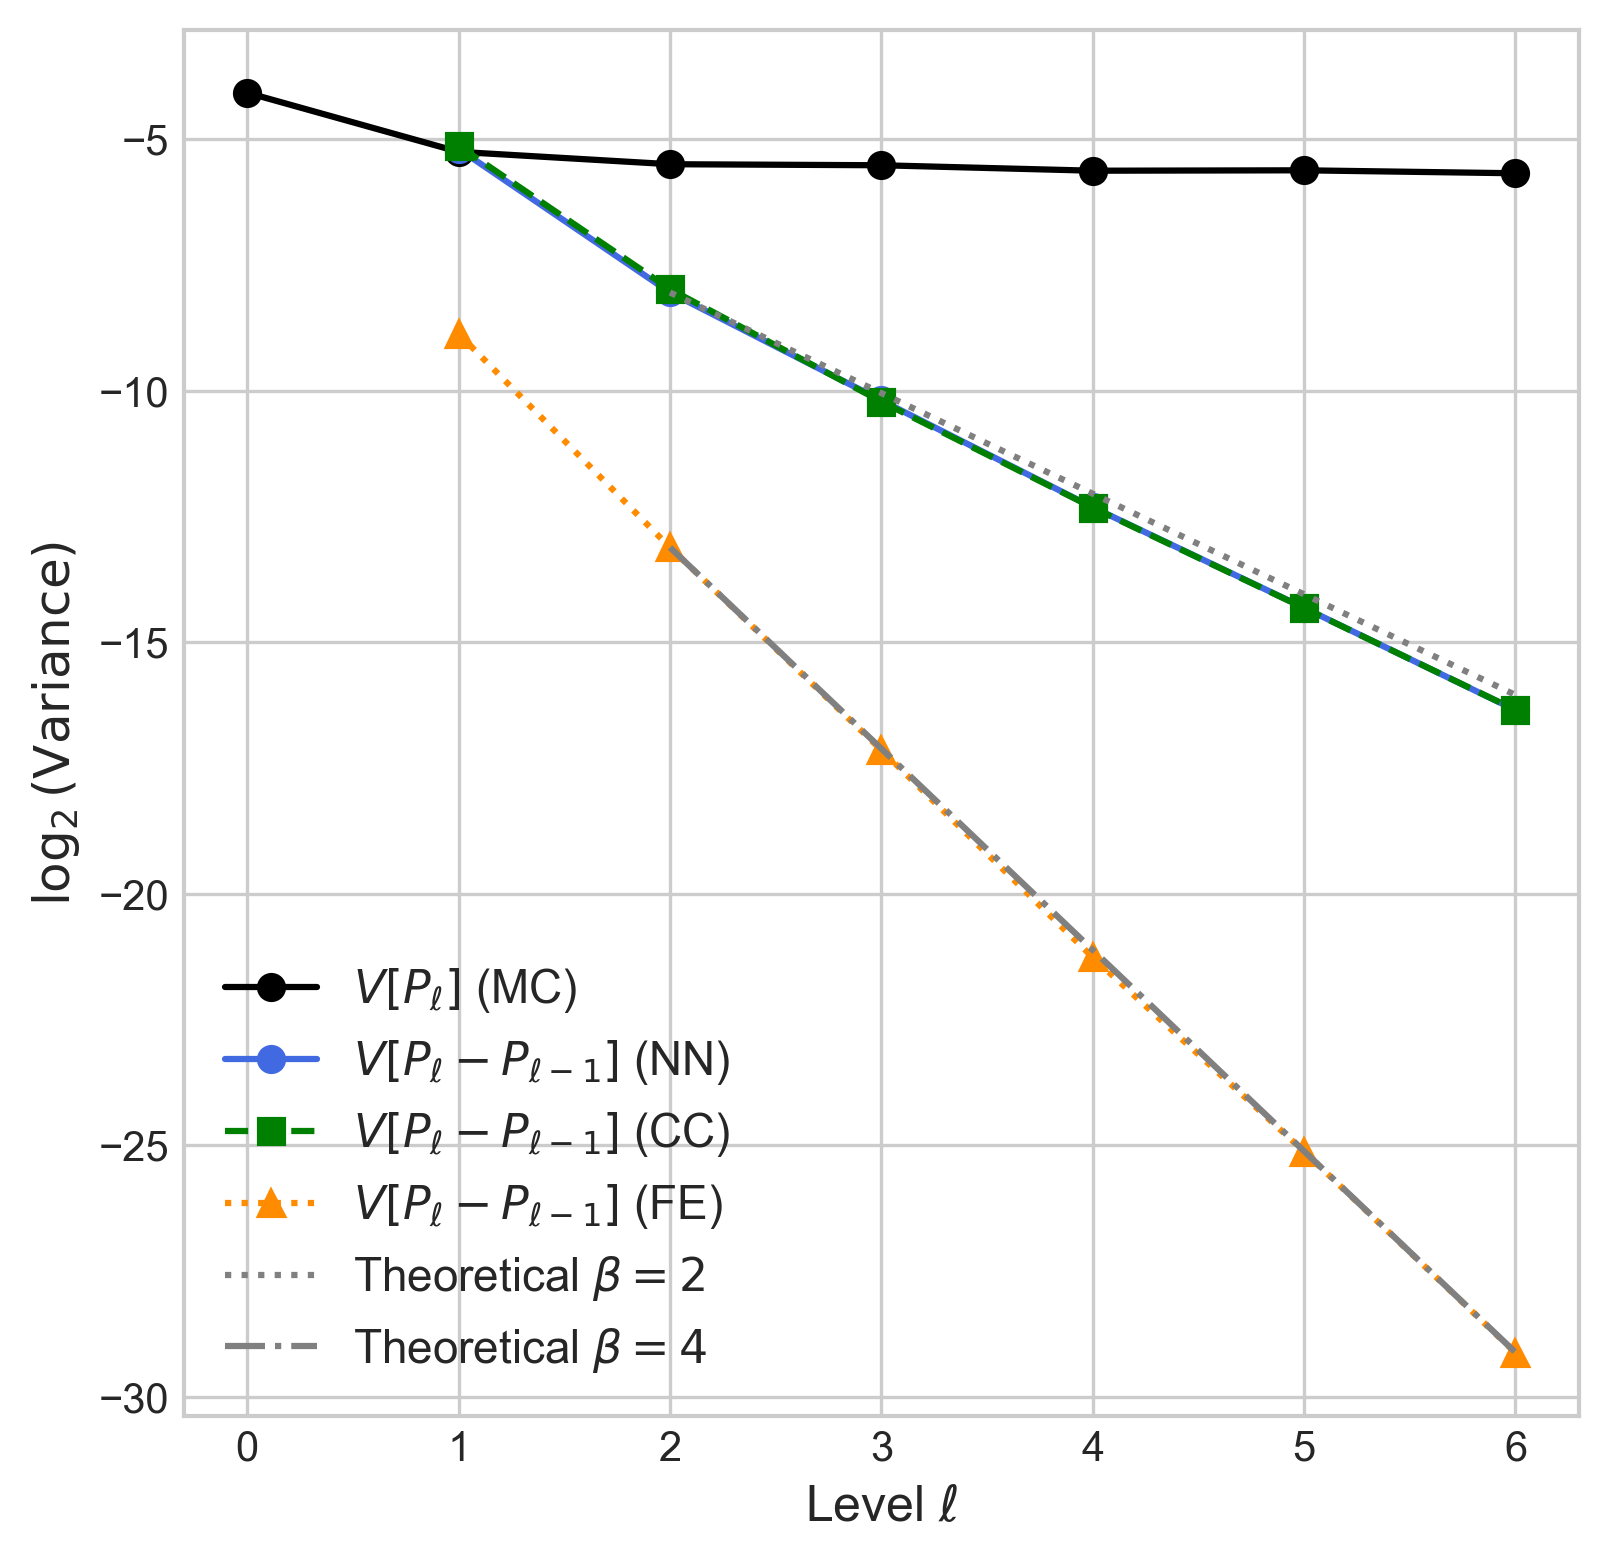
\includegraphics[width=\linewidth]{graphics/she_sq_amp_var_decay.png}
            \caption{MLMC variance decay ($\beta$).}
            \label{fig:variance_decay}
        \end{subfigure}
        \hfill
        \begin{subfigure}[b]{0.48\textwidth}
            \centering
            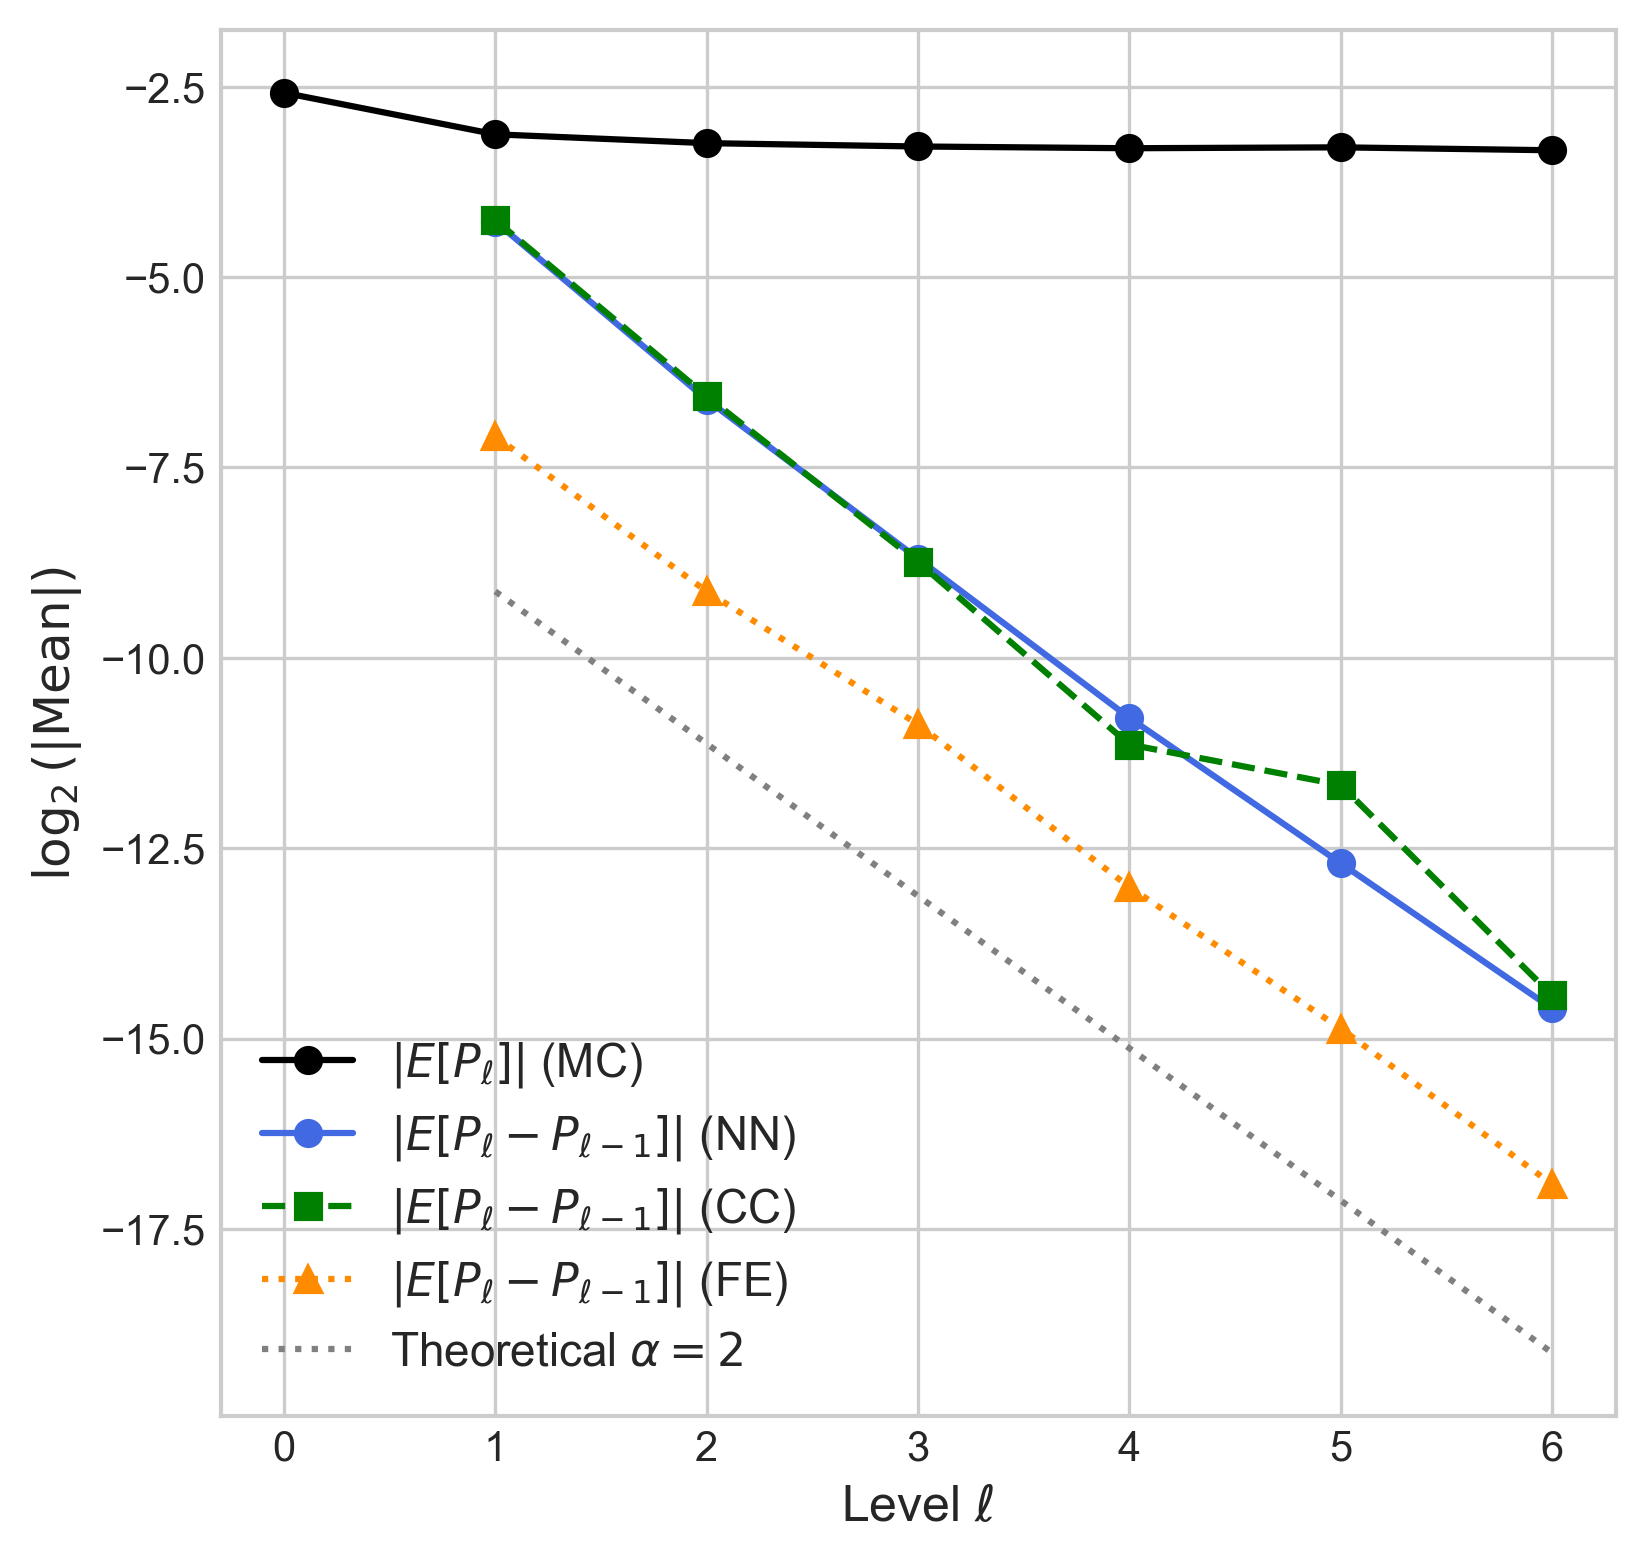
\includegraphics[width=\linewidth]{graphics/she_sq_amp_err_decay.png}
            \caption{Weak error convergence ($\alpha$).}
            \label{fig:mean_decay}
        \end{subfigure}
    \end{subfigure}
    \vspace{1cm}
    \begin{subfigure}{\textwidth}
        \centering
        \begin{subfigure}[b]{\textwidth}
            \centering
            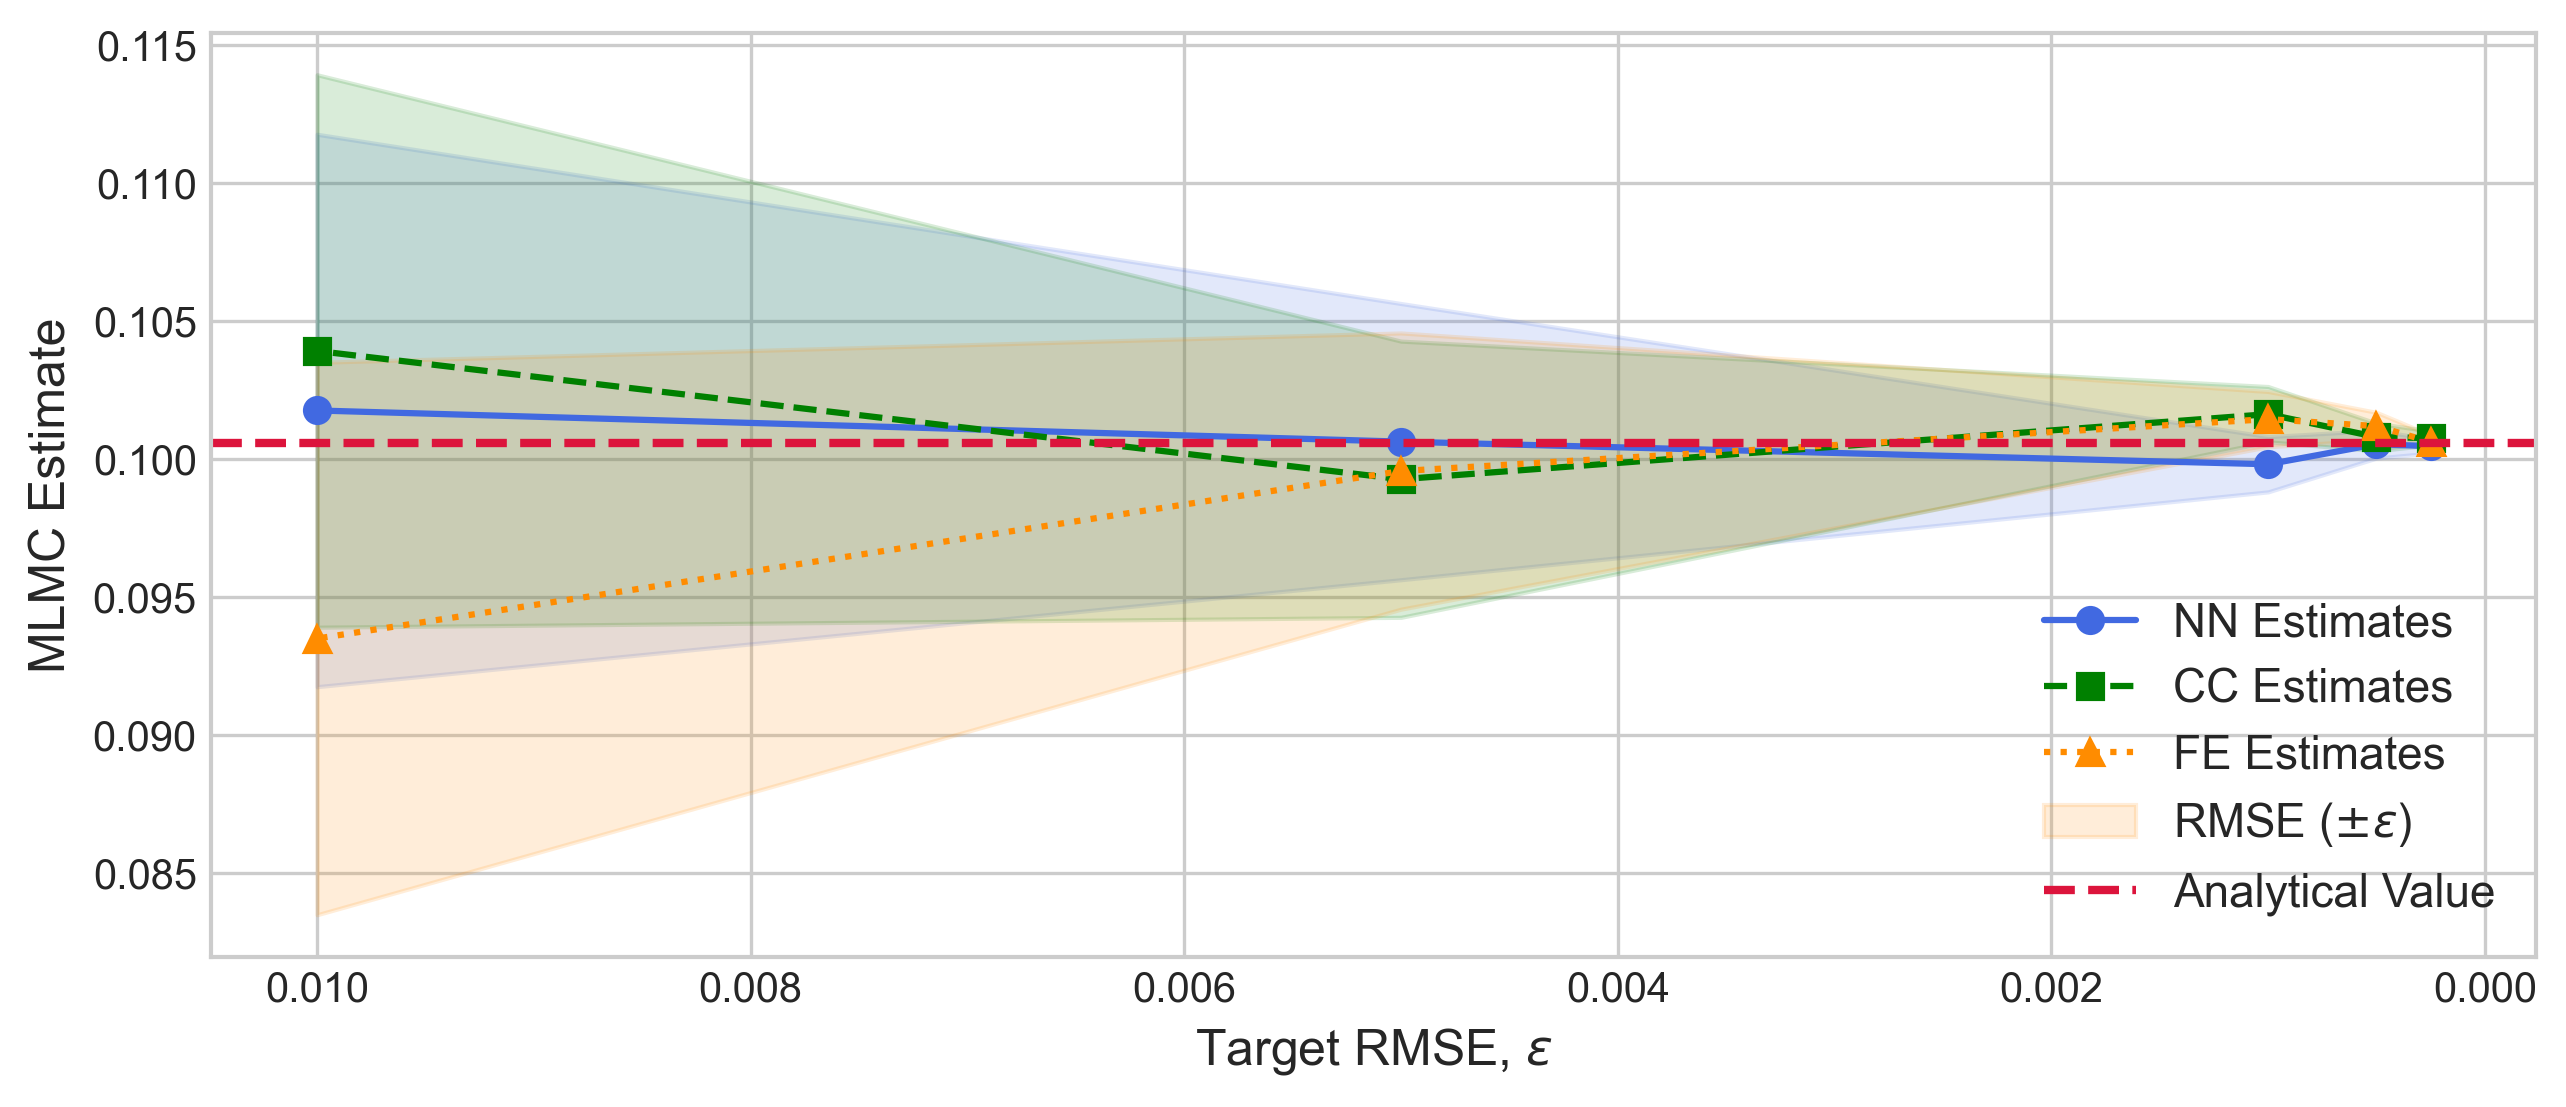
\includegraphics[width=0.7\linewidth]{graphics/she_sq_amp_conv.png}
            \caption{Final MLMC estimate vs. target RMSE ($\varepsilon$).}
            \label{fig:conv_vs_eps}
        \end{subfigure}
        \vspace{0.5cm}
        \begin{subfigure}[b]{\textwidth}
            \centering
            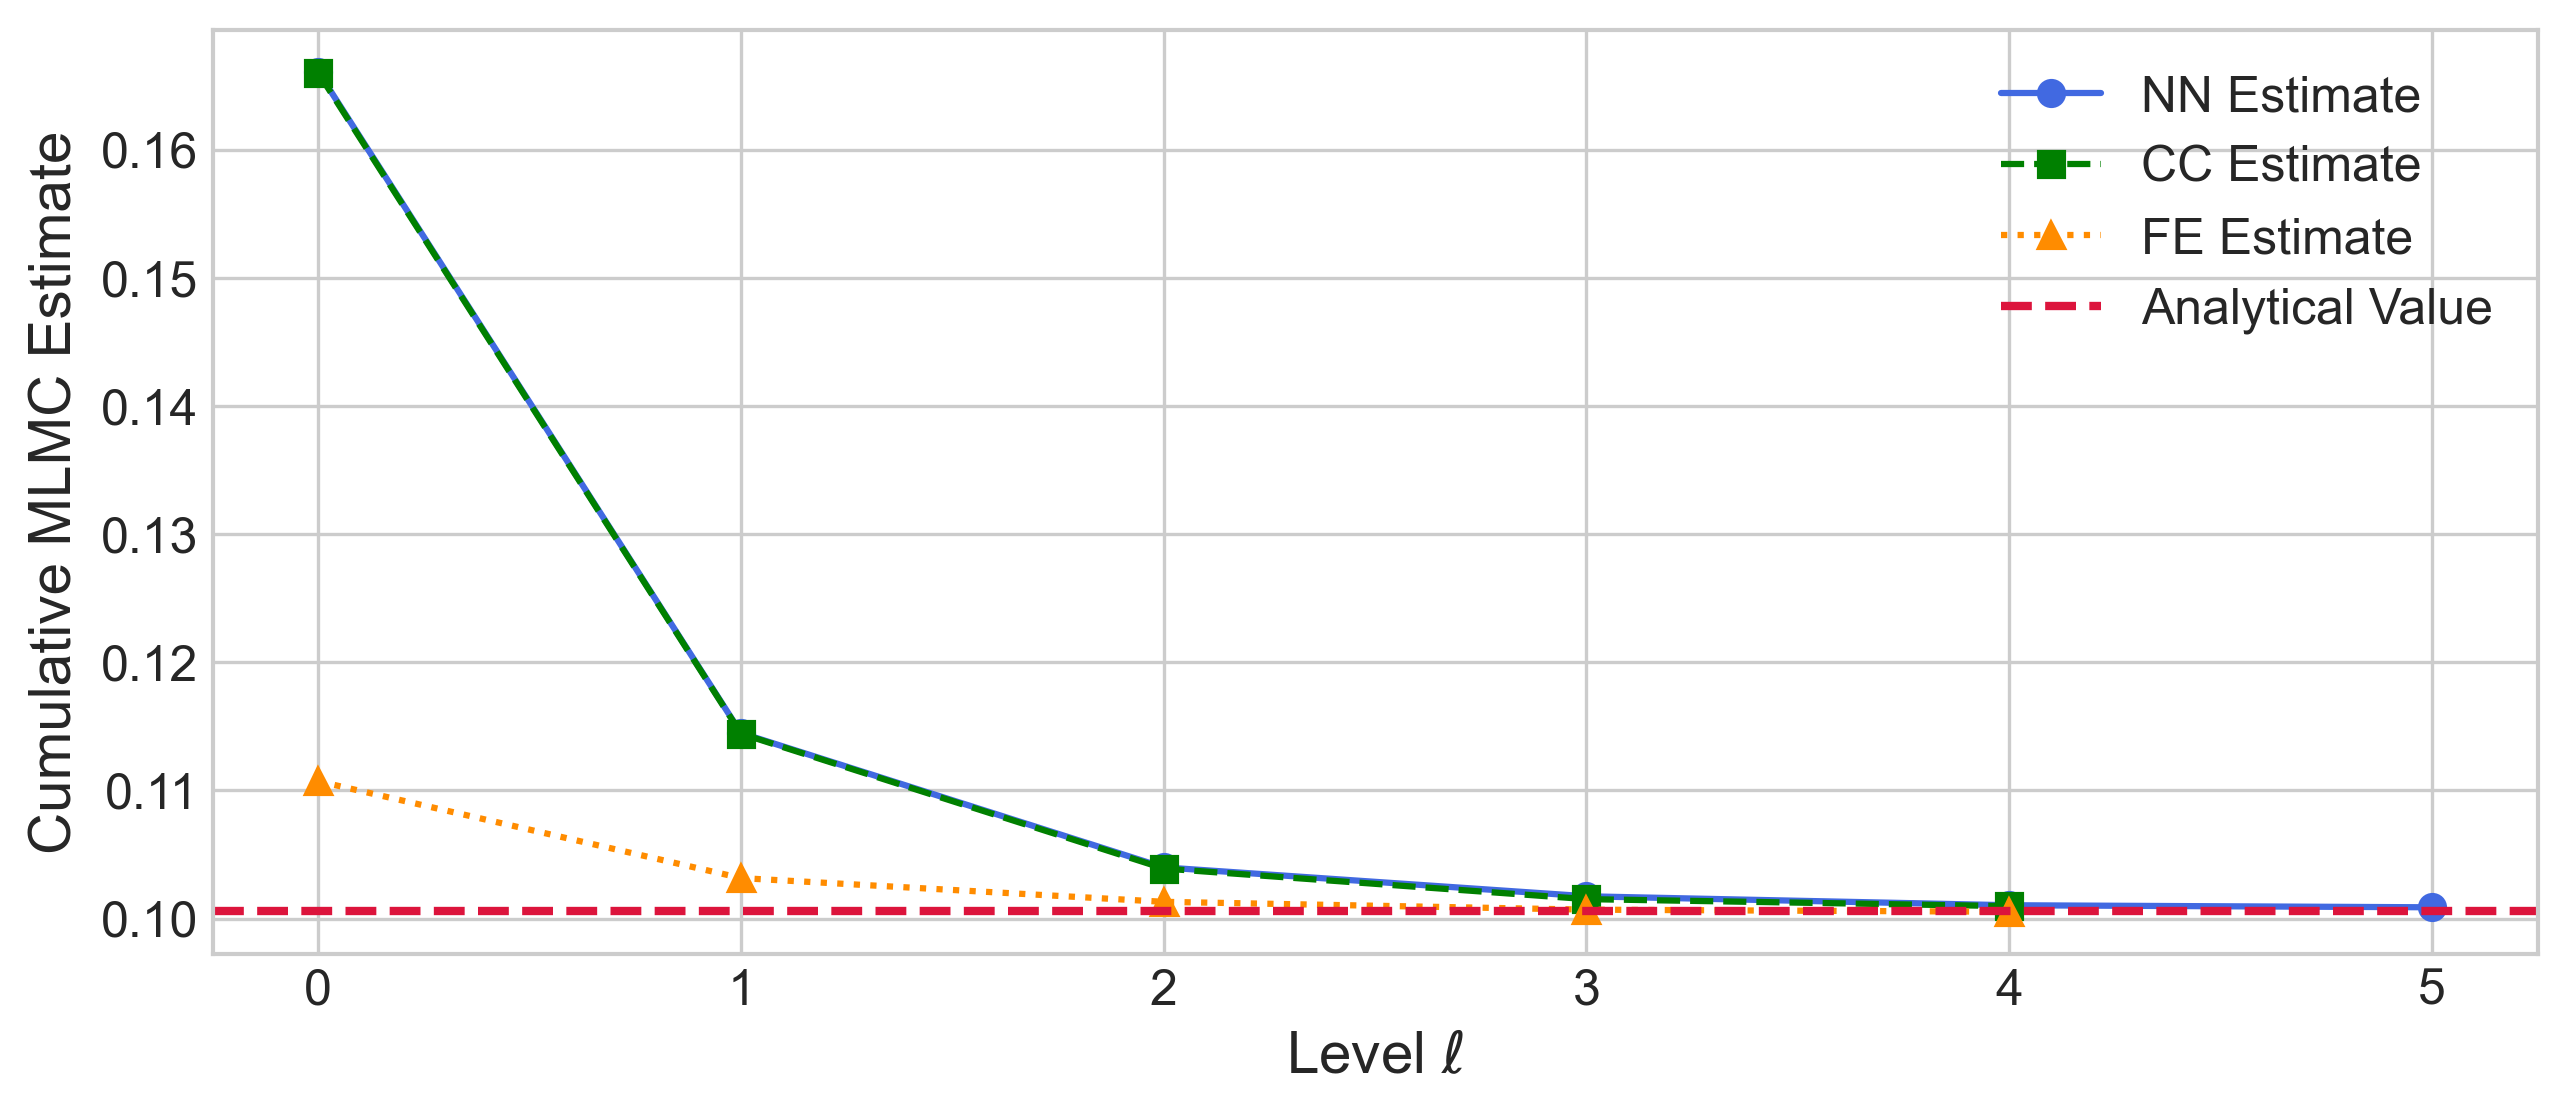
\includegraphics[width=0.7\linewidth]{graphics/she_sq_amp_cumconv.png}
            \caption{Cumulative estimate vs. level ($\ell$) for $\varepsilon=0.001$.}
            \label{fig:cumulative_conv}
        \end{subfigure}
    \end{subfigure}
    \caption{Validation and convergence plots for the MLMC implementation for the SHE, using the squared 
    amplitude of the first Fourier mode as our QoI.}
    \label{fig:she_validation_combined}
\end{figure}

\begin{table}[htbp]
    \centering
    \begin{tabular}{|l|c|c|r|}
        \hline
        \textbf{Coupling Method} & \textbf{$\alpha$} & \textbf{$\beta$} & \textbf{$\gamma$} \\
        \hline
        Nearest Neighbour & 2.0 & 2.07 & 3.02\\
        Central Coupling & 1.86 & 2.08 & 3.02 \\
        Finite Element & 1.96 & 4.0 & 3.0 \\
        \hline
    \end{tabular}
    \caption{Empirically estimated rates for the Squared Amplitude QoI.}
    \label{tab:she_decay_rates}
\end{table}


Figures \ref{fig:conv_vs_eps} and \ref{fig:cumulative_conv} 
show that the MLMC estimates for all three coupling strategies converge to the true 
value. 


The decay rate plots align with our theoretical predictions from Propositions 
\ref{prop:weak_error_for_fourier_mode} and \ref{prop:variance_decay_fourier}. 
The weak error for all methods, shown in Figure \ref{fig:mean_decay},
converges with a rate of $\alpha \approx 2$, consistent with 
the expected $\mathcal{O}((\Delta x)^2)$ convergence.

The variance decay plot in Figure \ref{fig:variance_decay} highlights the critical 
difference between the coupling strategies. The NN and CC methods 
both exhibit a variance decay of $\beta \approx 2$, which aligns with the theoretical rate 
for imperfectly correlated processes. In contrast, the FE coupling 
method achieves a much faster decay rate of $\beta \approx 4$. This confirms that the 
mathematically-grounded coupling derived from the FEM basis functions achieves the optimal
rate for this quantity of interest.




\begin{figure}[htbp]
    \centering
    \begin{subfigure}{\textwidth}
        \centering
        \begin{subfigure}[b]{0.48\textwidth}
            \centering
            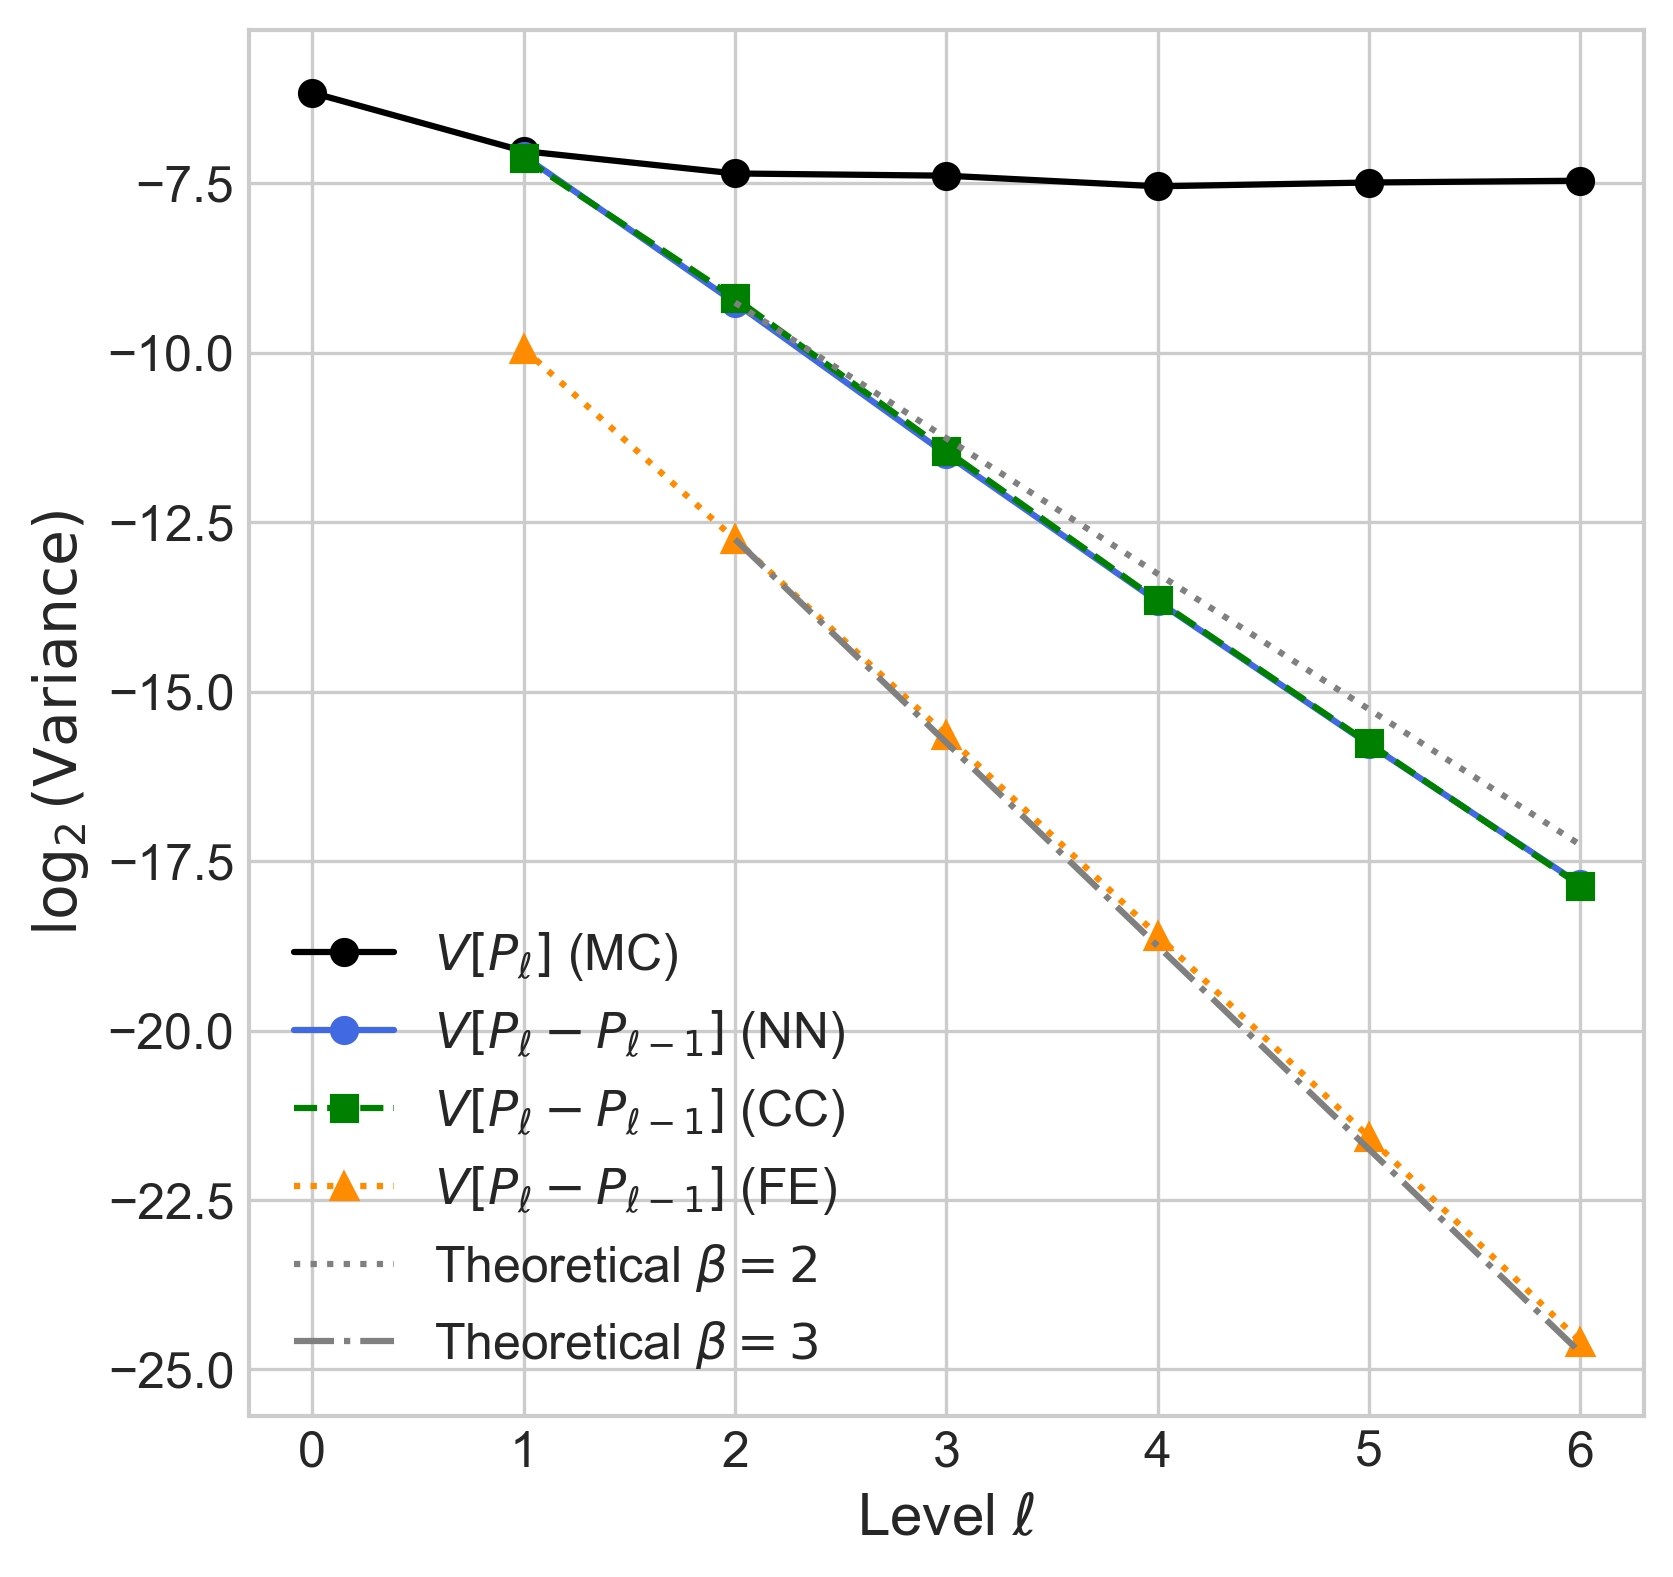
\includegraphics[width=\linewidth]{graphics/she_energy_var_decay.png}
            \caption{MLMC variance decay ($\beta$).}
            \label{fig:variance_decay}
        \end{subfigure}
        \hfill
        \begin{subfigure}[b]{0.48\textwidth}
            \centering
            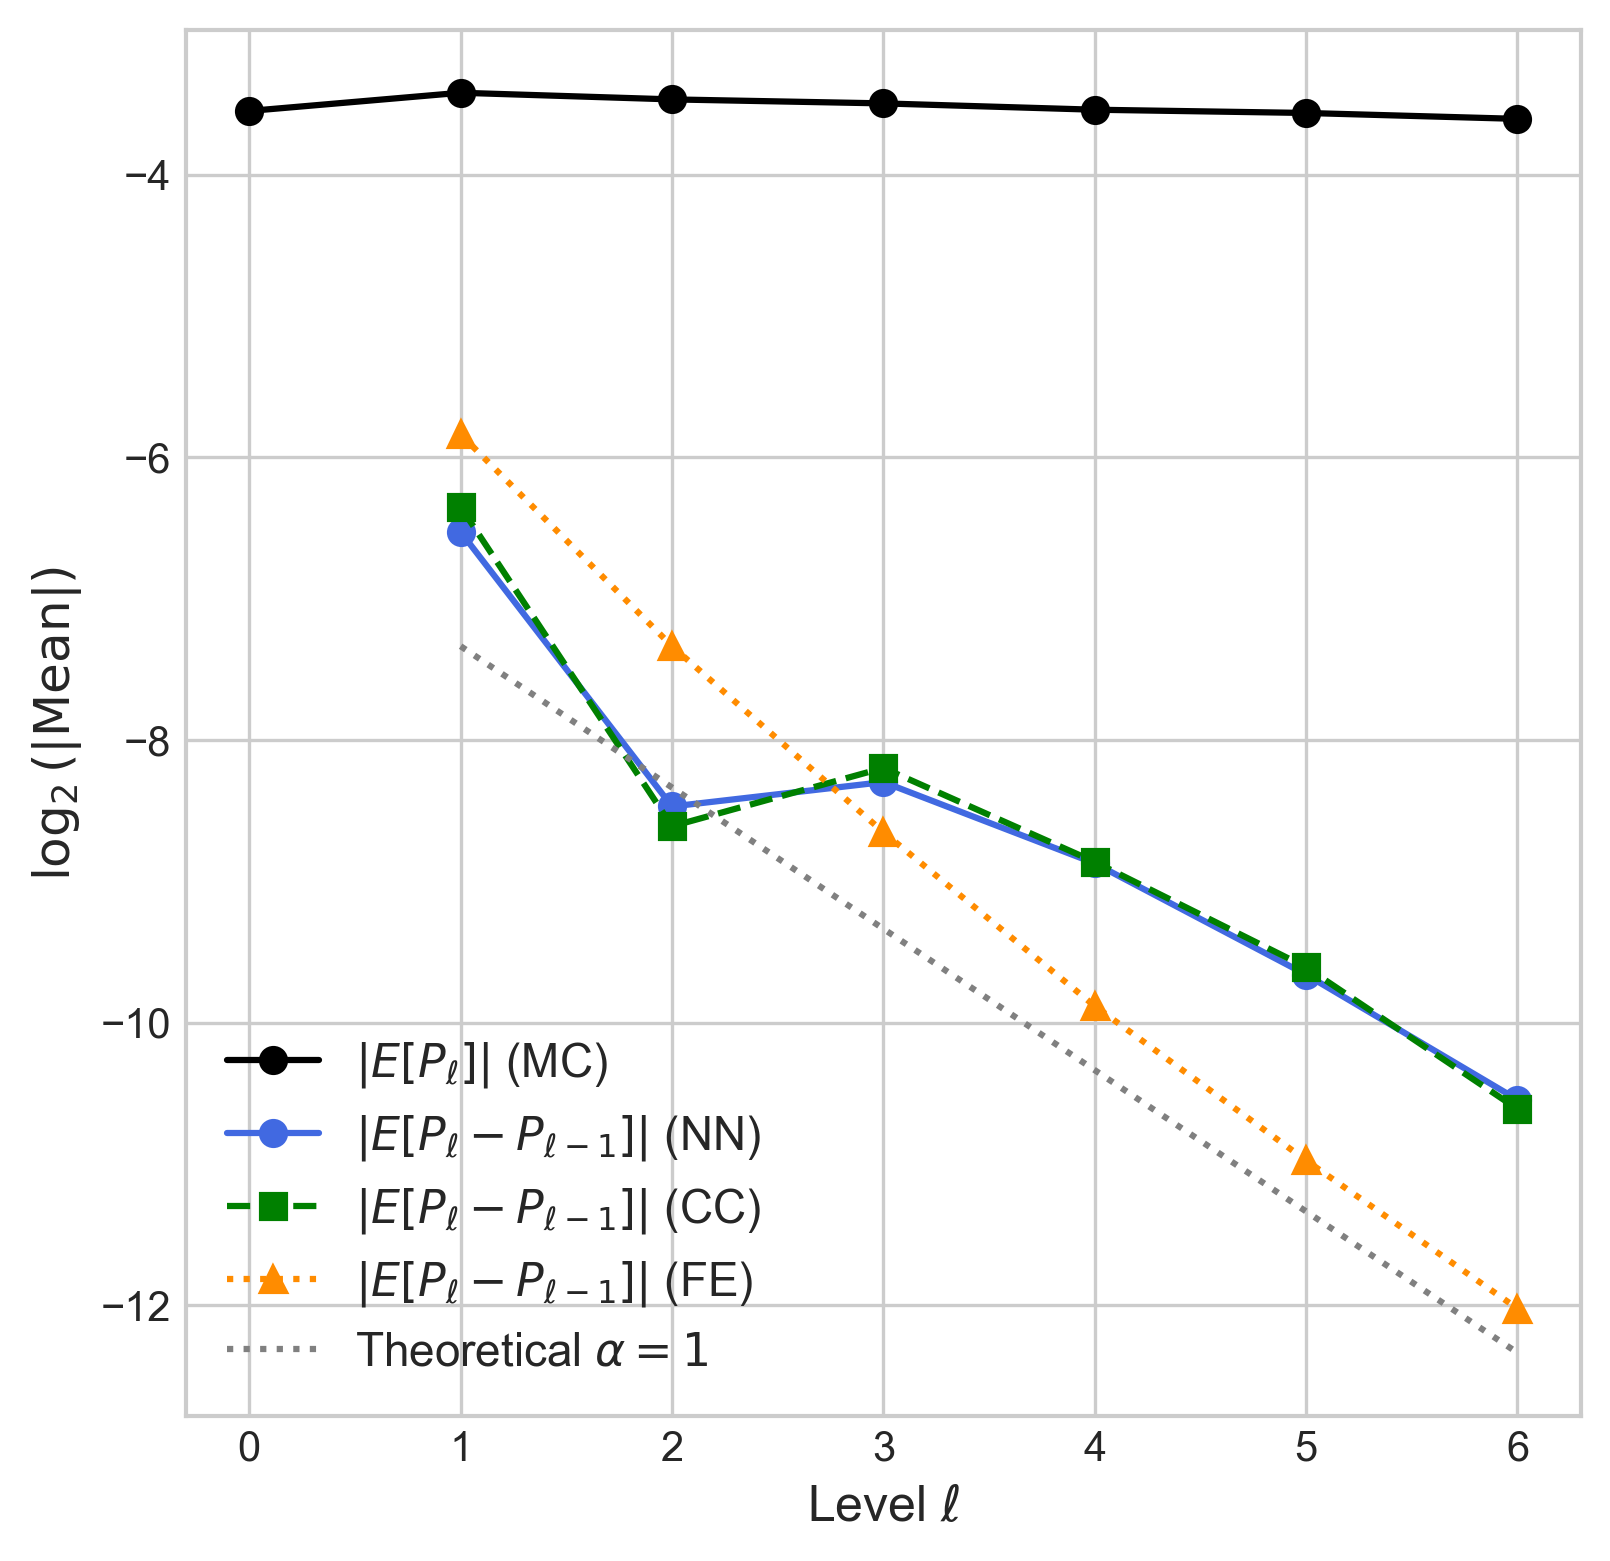
\includegraphics[width=\linewidth]{graphics/she_energy_err_decay.png}
            \caption{Weak error convergence ($\alpha$).}
            \label{fig:mean_decay}
        \end{subfigure}
    \end{subfigure}
    \vspace{1cm}
    \begin{subfigure}{\textwidth}
        \centering
        \begin{subfigure}[b]{\textwidth}
            \centering
            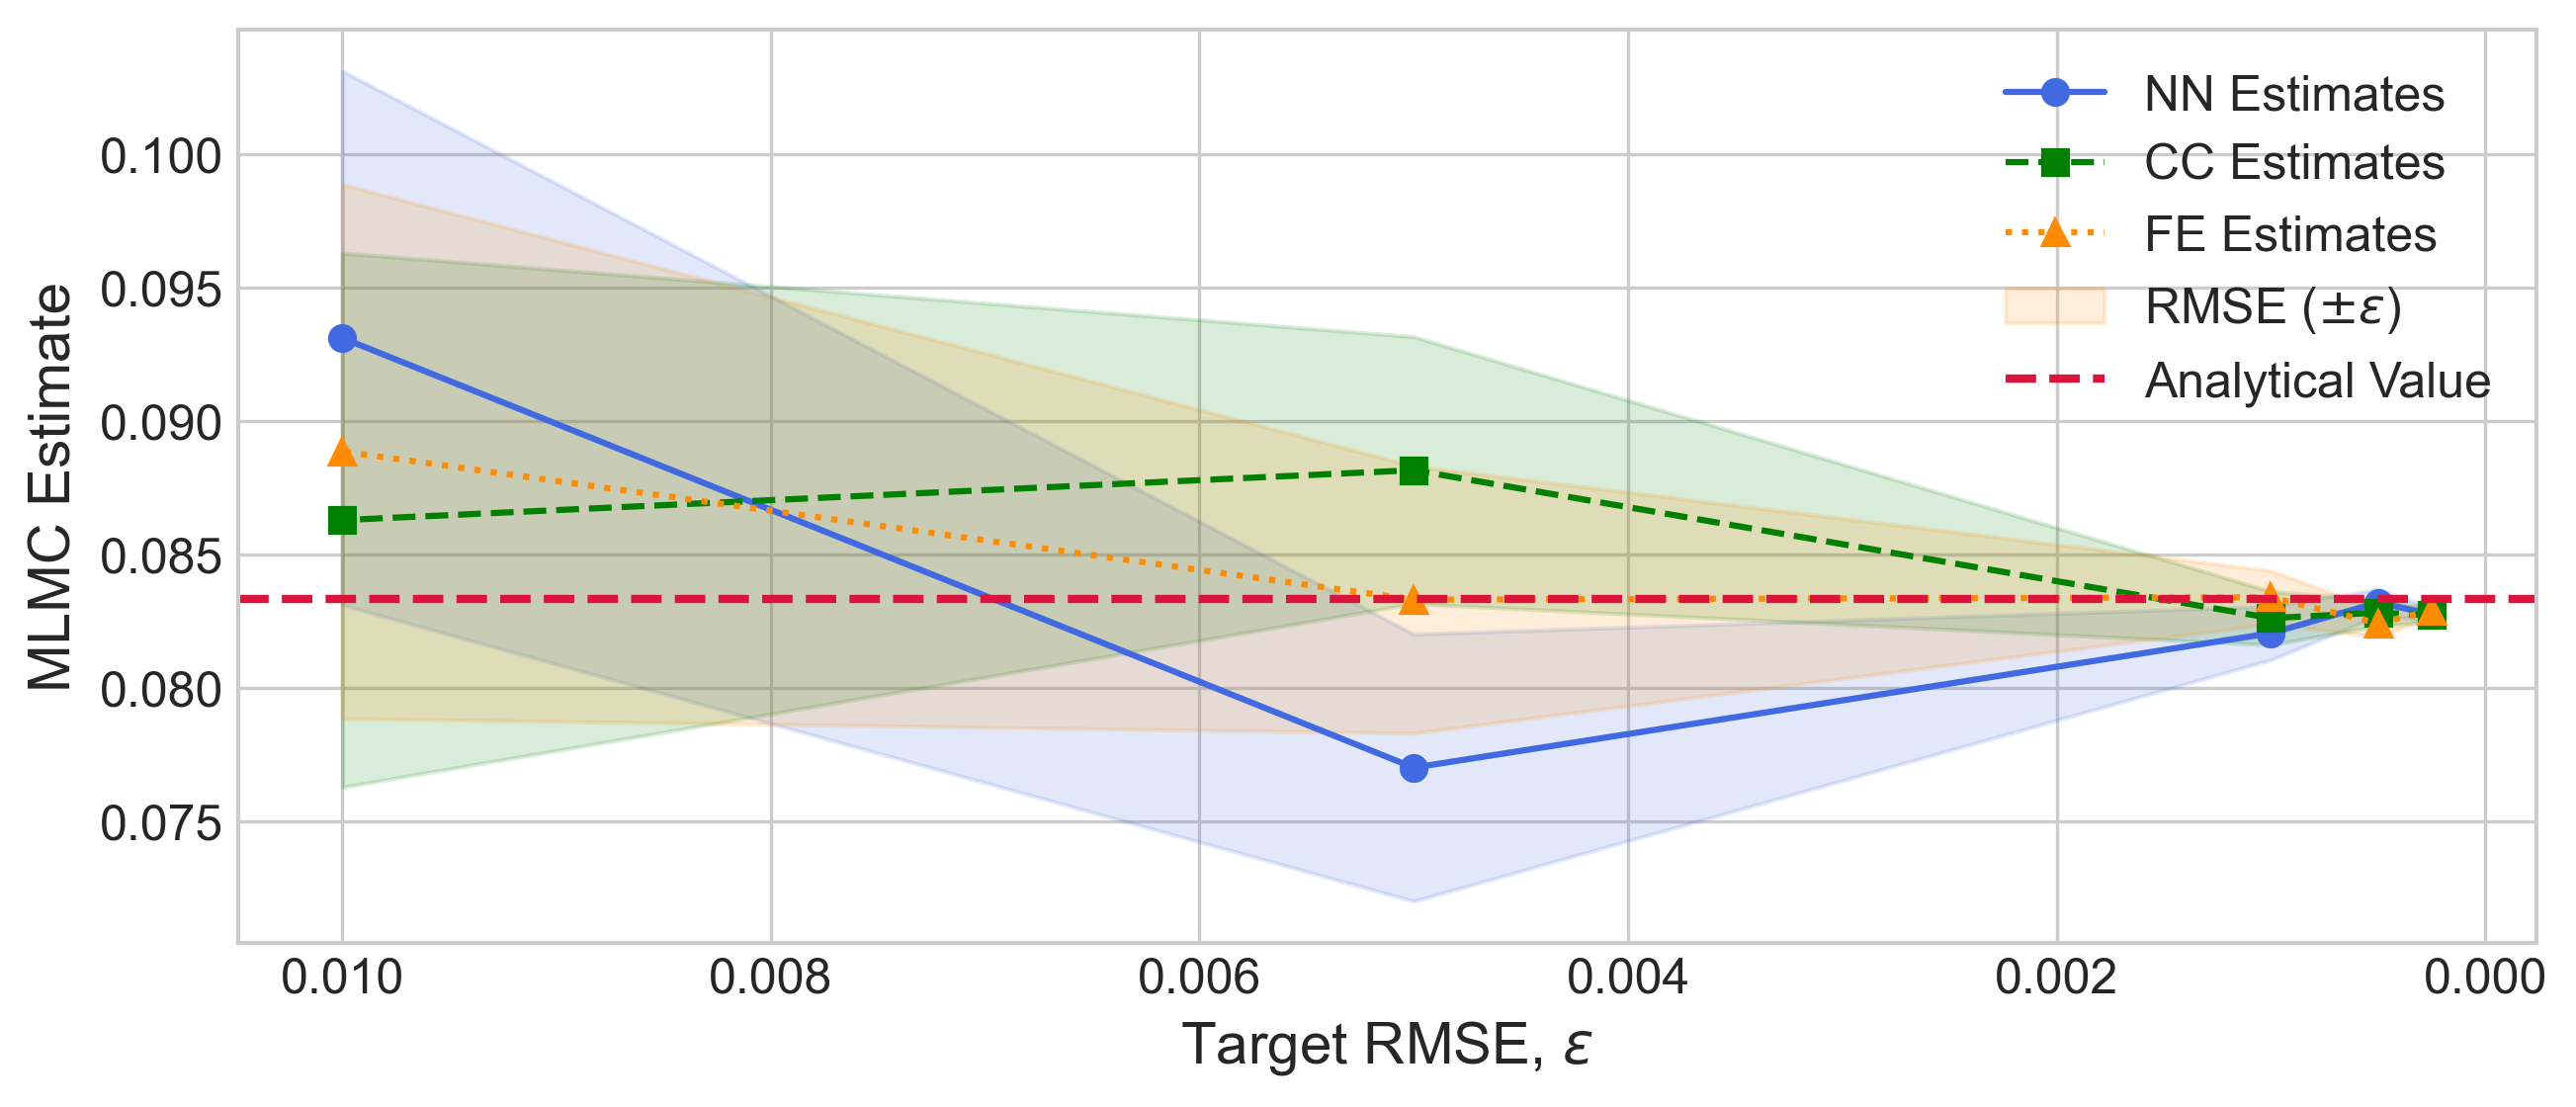
\includegraphics[width=0.7\linewidth]{graphics/she_energy_conv.png}
            \caption{Final MLMC estimate vs. target RMSE ($\varepsilon$).}
            \label{fig:conv_vs_eps}
        \end{subfigure}
        \vspace{0.5cm}
        \begin{subfigure}[b]{\textwidth}
            \centering
            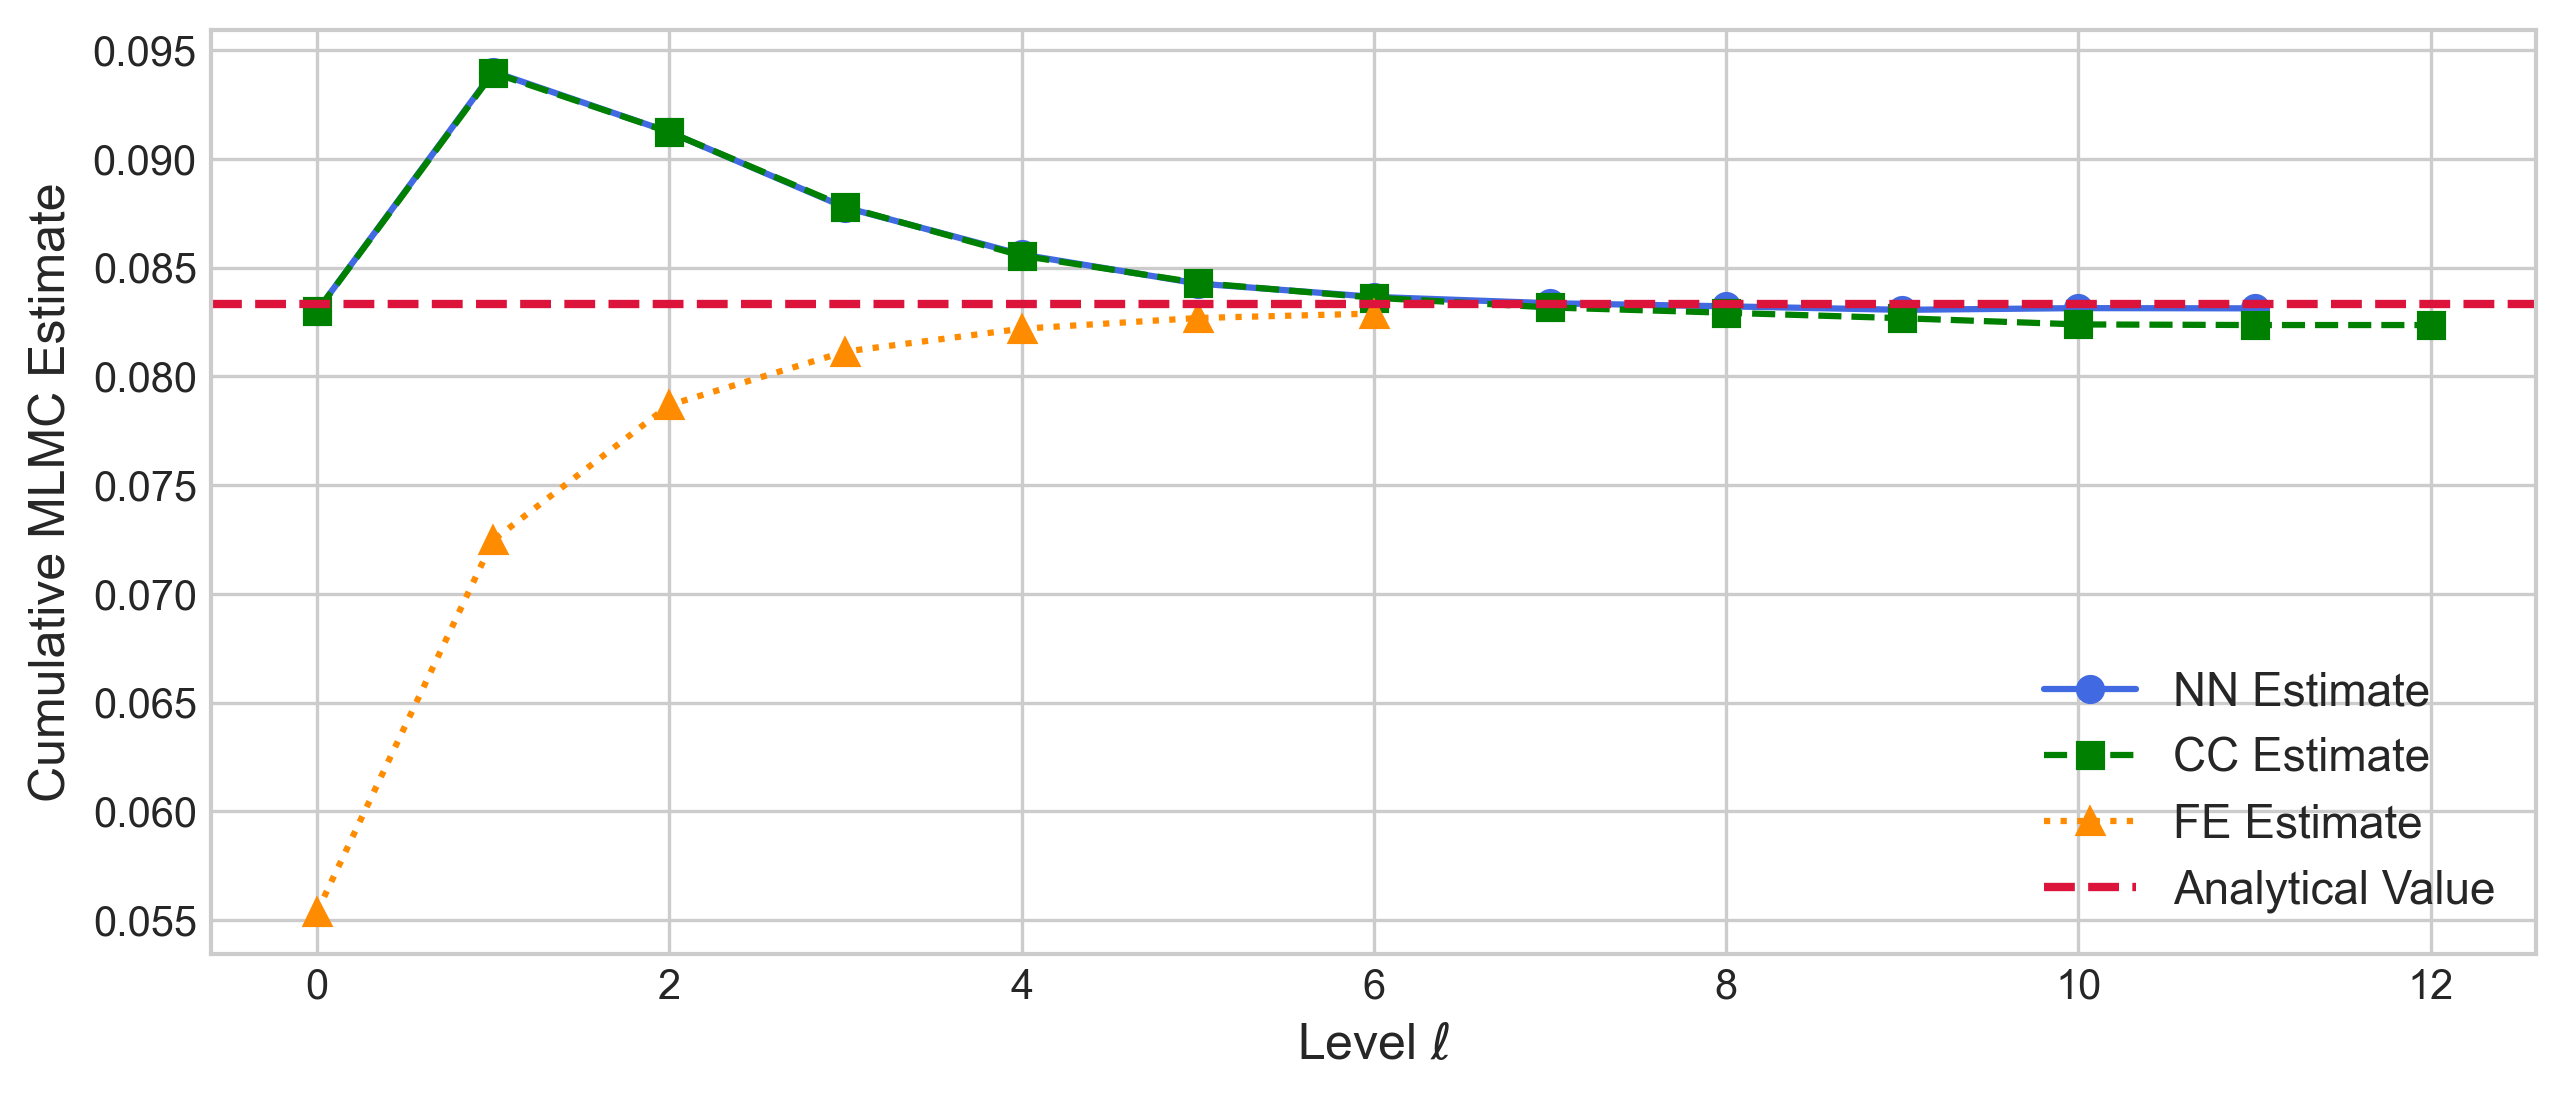
\includegraphics[width=0.7\linewidth]{graphics/she_energy_cumconv.png}
            \caption{Cumulative estimate vs. level ($\ell$) for $\varepsilon=0.001$.}
            \label{fig:cumulative_conv}
        \end{subfigure}
    \end{subfigure}
    \caption{Validation and convergence plots for the MLMC implementation for the SHE, evaluating
    the energy.}
    \label{fig:she_validation_combined}
\end{figure}

\section{Dean-Kawasaki Validation}\label{sec:dk_validation}

\subsection{Dean-Kawasaki Implementation}\label{sec:dk_implementation} 
We now present the Dean-Kawasaki problem considered and the finite-difference scheme,
following \cite{cornalba2025multilevel}, and our MLMC 
implementation.
We consider the Dean-Kawasaki equation on a one dimensional torus
$\Omega=[0,2\pi)$ with periodic boundary conditions and final time $T>0$.
The particle number is denoted $N_p$. The density 
field $\rho$ evolves according to

\begin{align}
\frac{\partial \rho(t,x)}{\partial t}
&= \frac{1}{2}\,\frac{\partial^2 \rho(t,x)}{\partial x^2}
\;+\; N_p^{-1/2}\,\frac{\partial \!\left(\sqrt{\rho(t,x)}\,\xi(t,x)\right)}{\partial x},
&& (t,x)\in (0,T]\times [0, 2\pi),
\label{eq:dk_spde_problem}\\[4pt]
\rho(0,x)
&= Z_0\!\left(1+\frac{1}{\sqrt{2\pi}}
\,\exp\!\left(-\tfrac{1}{2}\,\sin^2\!\big(x-\tfrac{\pi}{2}\big)\right)\right),
&& x\in\Omega, \nonumber\\
\rho(t,0) &= \rho(t,2\pi), &&t \in [0,T], \nonumber
\end{align}
where $\xi$ is space-time white noise and $Z_0 \approx 
0.12$ is a normalisation constant.

We discretise $\Omega$ with a uniform grid of spacing 
$\Delta x, \Delta t$ and denote by $\rho_j^n$ the approximation
to $\rho(t_n, x_j)$ at time $t_n = n \Delta t$ and position $x_j = 
\Delta x$.

\begin{align}
\rho_j^{\,n+1}
&= \rho_j^{\,n}
\;+\; \tfrac{\lambda}{2}\,\bigl(\rho_{j+1}^{\,n}-2\rho_j^{\,n}+\rho_{j-1}^{\,n}\bigr)
\;+\; \tfrac{1}{\sqrt{N_p}}\,
\frac{F_{j+1}^{\,n}-F_{j-1}^{\,n}}{2\Delta x}, \label{eq:dk_fd}\\[4pt]
F_j^n &:= \sqrt{[\rho_j^n]_+}\,\Delta W_j^n, \qquad
\Delta W_j^n \overset{\text{i.i.d.}}{\sim} \mathcal{N}\!\left(0,\ \tfrac{\Delta t}{\Delta x}\right).
\nonumber
\end{align}

Our quantity of interest is the expected squared mean field fluctuations
in the $\sin(x)$ mode at final time $T$, namely

\begin{equation}\label{eq:dk_qoi}
P = \mathbb{E}\!\left[\,N_p \left(\int_0^{2\pi} 
\big(\rho(T,x)-\bar{\rho}(T,x)\big)\,\sin(x)\,\mathrm{d}x\right)^{\!2}\right],
\end{equation}
where $\bar\rho$ denotes the deterministic mean-field solution.

In the discrete setting we approximate this by
\begin{equation}
P \;=\; N_p \left( \big(\boldsymbol{\rho}^N - \boldsymbol{\bar\rho}^N,\ 
\sin(x_h)\big)_h \right)^{\!2},
\end{equation}

To compute $P$, we update in parallel the 
deterministic mean-field 
solution $\bar\rho$ via an explicit finite difference scheme for the 
heat equation.

Our MLMC implementation is performed in the same manner as that 
used for the Stochastic Heat Equation,
We set $\Delta x_\ell = 2 \pi / 2^{l + 1}$, $\lambda = \frac{1}{4}$
and set $\Delta t = \lambda (\Delta x)^2$, ensuring stability 
\cite{cornalba2025multilevel}.
For our quantitiy of interest, we take $T=0.25$.

For coupling methods, we implement the NN and CC methods outlined in 
Section \ref{sec:she_scheme_mlmc_imp}. The NN method is 
used to replicate the results from Cornalba and Fischer \cite{cornalba2025multilevel}.
We then compare this with the proposed CC method to assess 
whether the symmetric coupling provides any tangible performance 
improvements.

\subsection{Dean-Kawasaki Validation}\label{sec:dk_validation}

We now verify that our implementation converges. We obtained an estimate of the true 
value of \eqref{eq:dk_qoi} via MC simulation, and now verify convergence 
of our implementation across a range of accuracies, 
$\varepsilon \in \{0.001, 0.005, 0.01, 0.05\}$. We also again 
analyse variance and error decay.

\begin{table}[htbp]
    \centering
    \begin{tabular}{|l|c|c|r|}
        \hline
        \textbf{Coupling Method} & \textbf{$\alpha$} & \textbf{$\beta$} & \textbf{$\gamma$} \\
        \hline
        Nearest Neighbour & 2.11 & 1.95 & 3.0\\
        Central Coupling & 1.95 & 1.95 & 2.98 \\
        \hline
    \end{tabular}
    \caption{Empirically estimated rates for the DK QoI.}
    \label{tab:energy_decay_rates}
\end{table}

\begin{figure}[htbp]
    \centering
    \begin{subfigure}{\textwidth}
        \centering
        \begin{subfigure}[b]{0.48\textwidth}
            \centering
            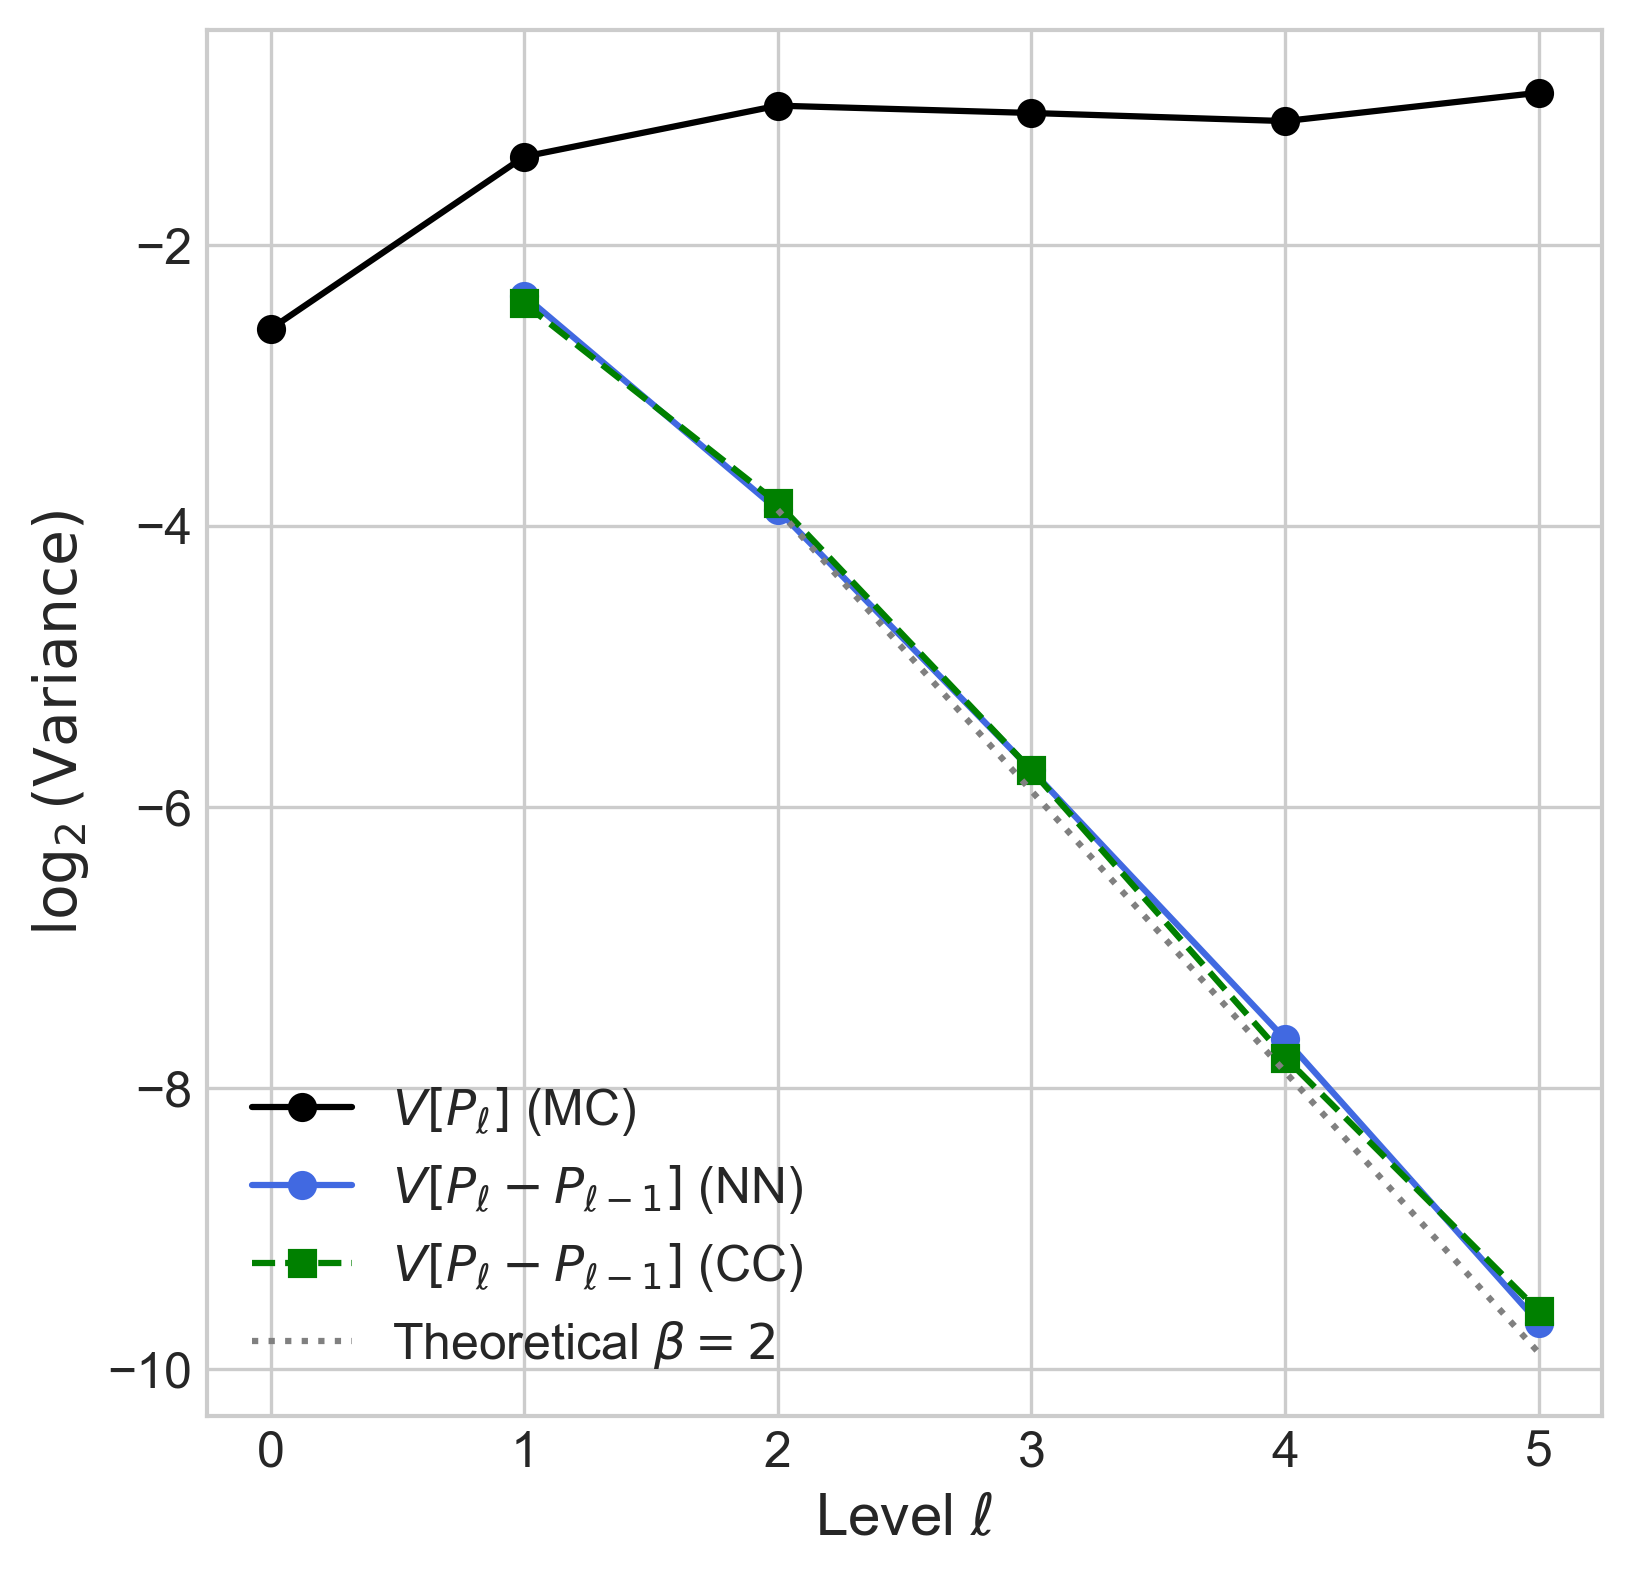
\includegraphics[width=\linewidth]{graphics/dk_var_decay.png}
            \caption{MLMC variance decay ($\beta$).}
            \label{fig:variance_decay}
        \end{subfigure}
        \hfill
        \begin{subfigure}[b]{0.48\textwidth}
            \centering
            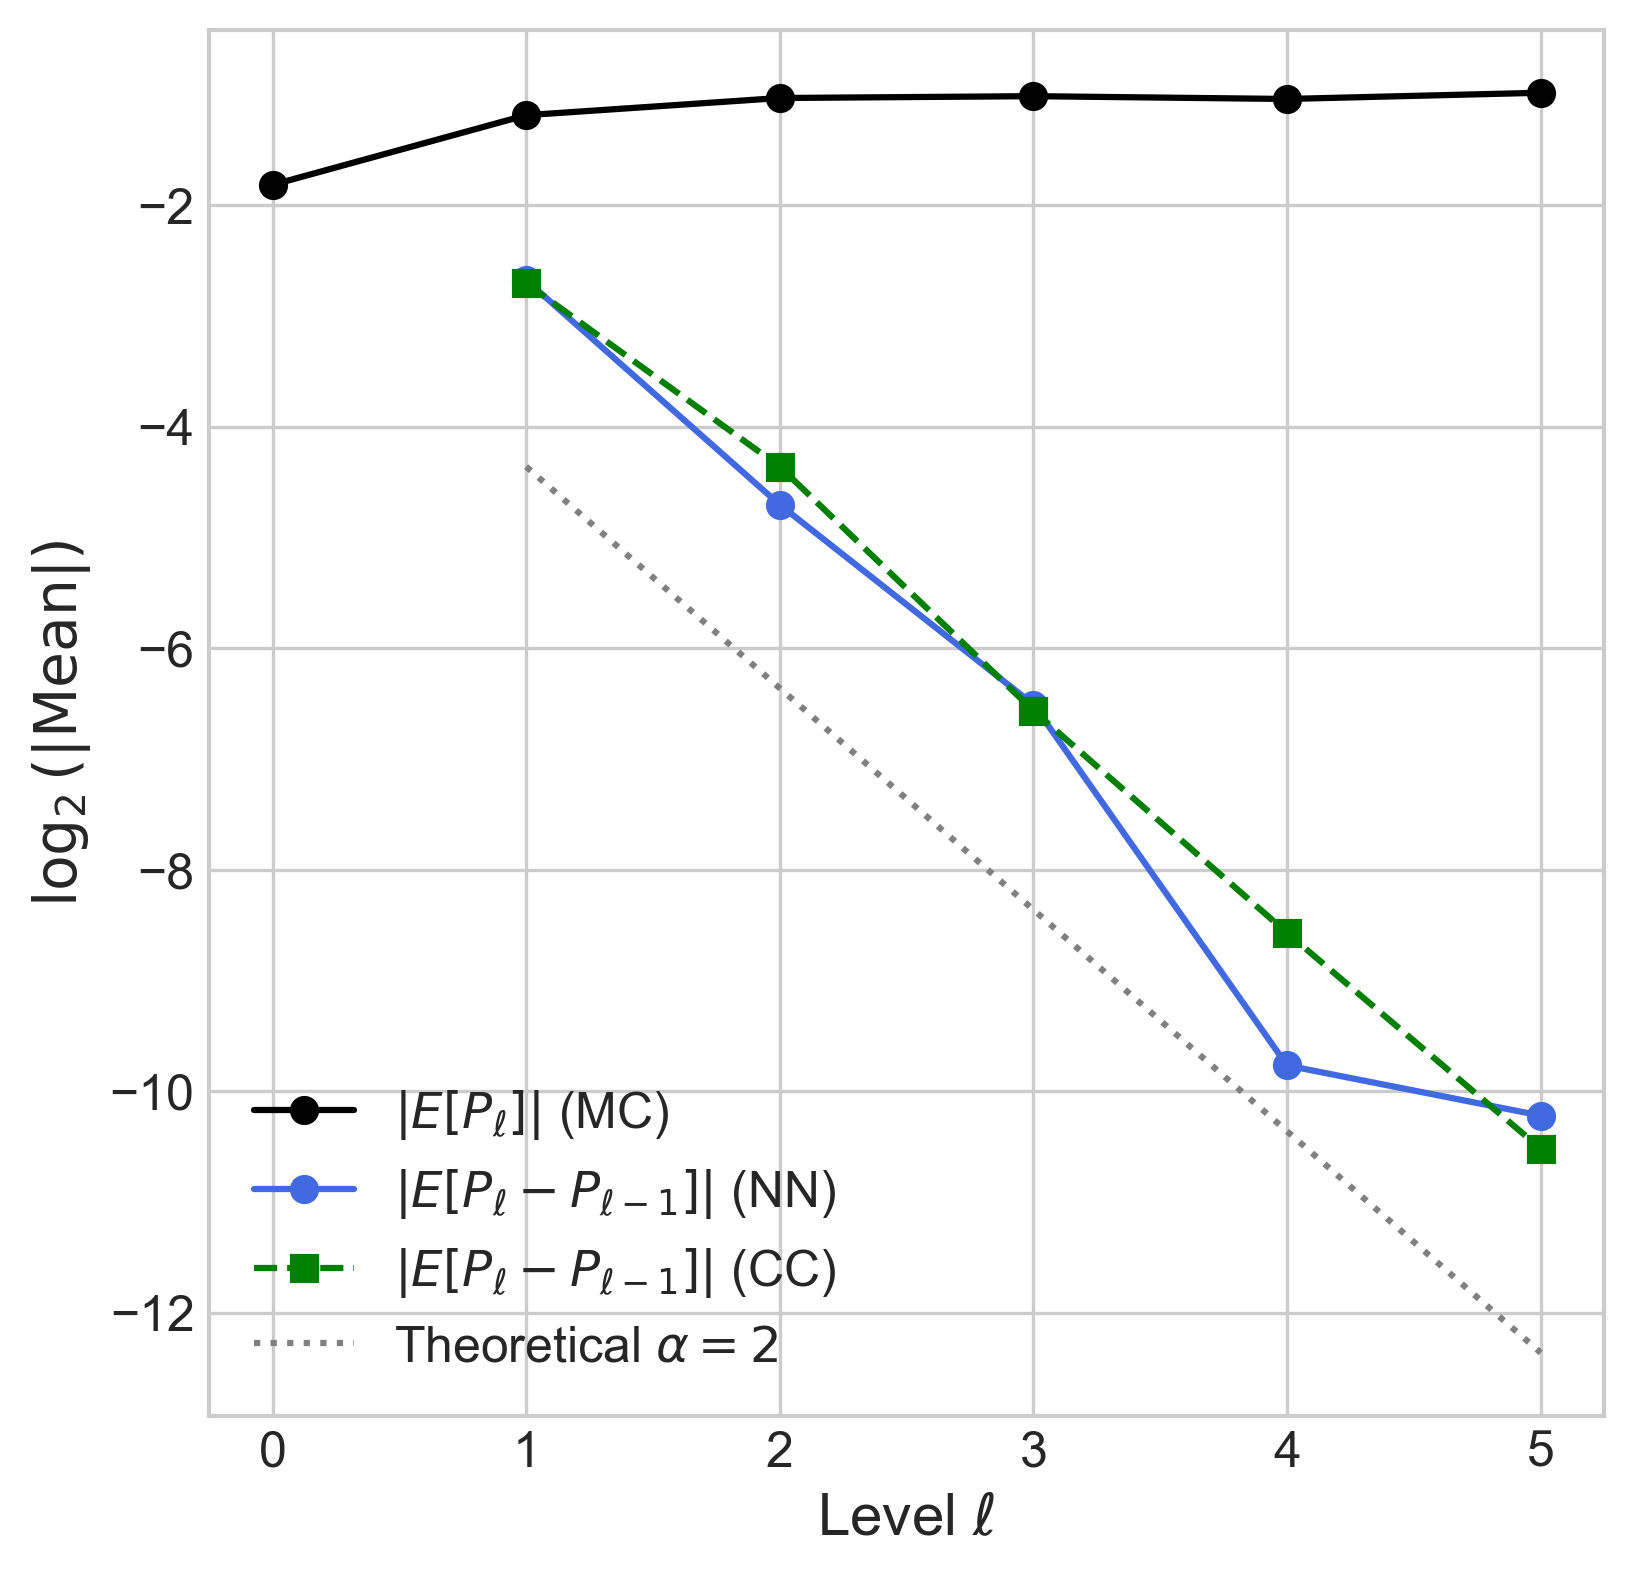
\includegraphics[width=\linewidth]{graphics/dk_err_decay.png}
            \caption{Weak error convergence ($\alpha$).}
            \label{fig:mean_decay}
        \end{subfigure}
    \end{subfigure}
    \vspace{1cm}
    \begin{subfigure}{\textwidth}
        \centering
        \begin{subfigure}[b]{\textwidth}
            \centering
            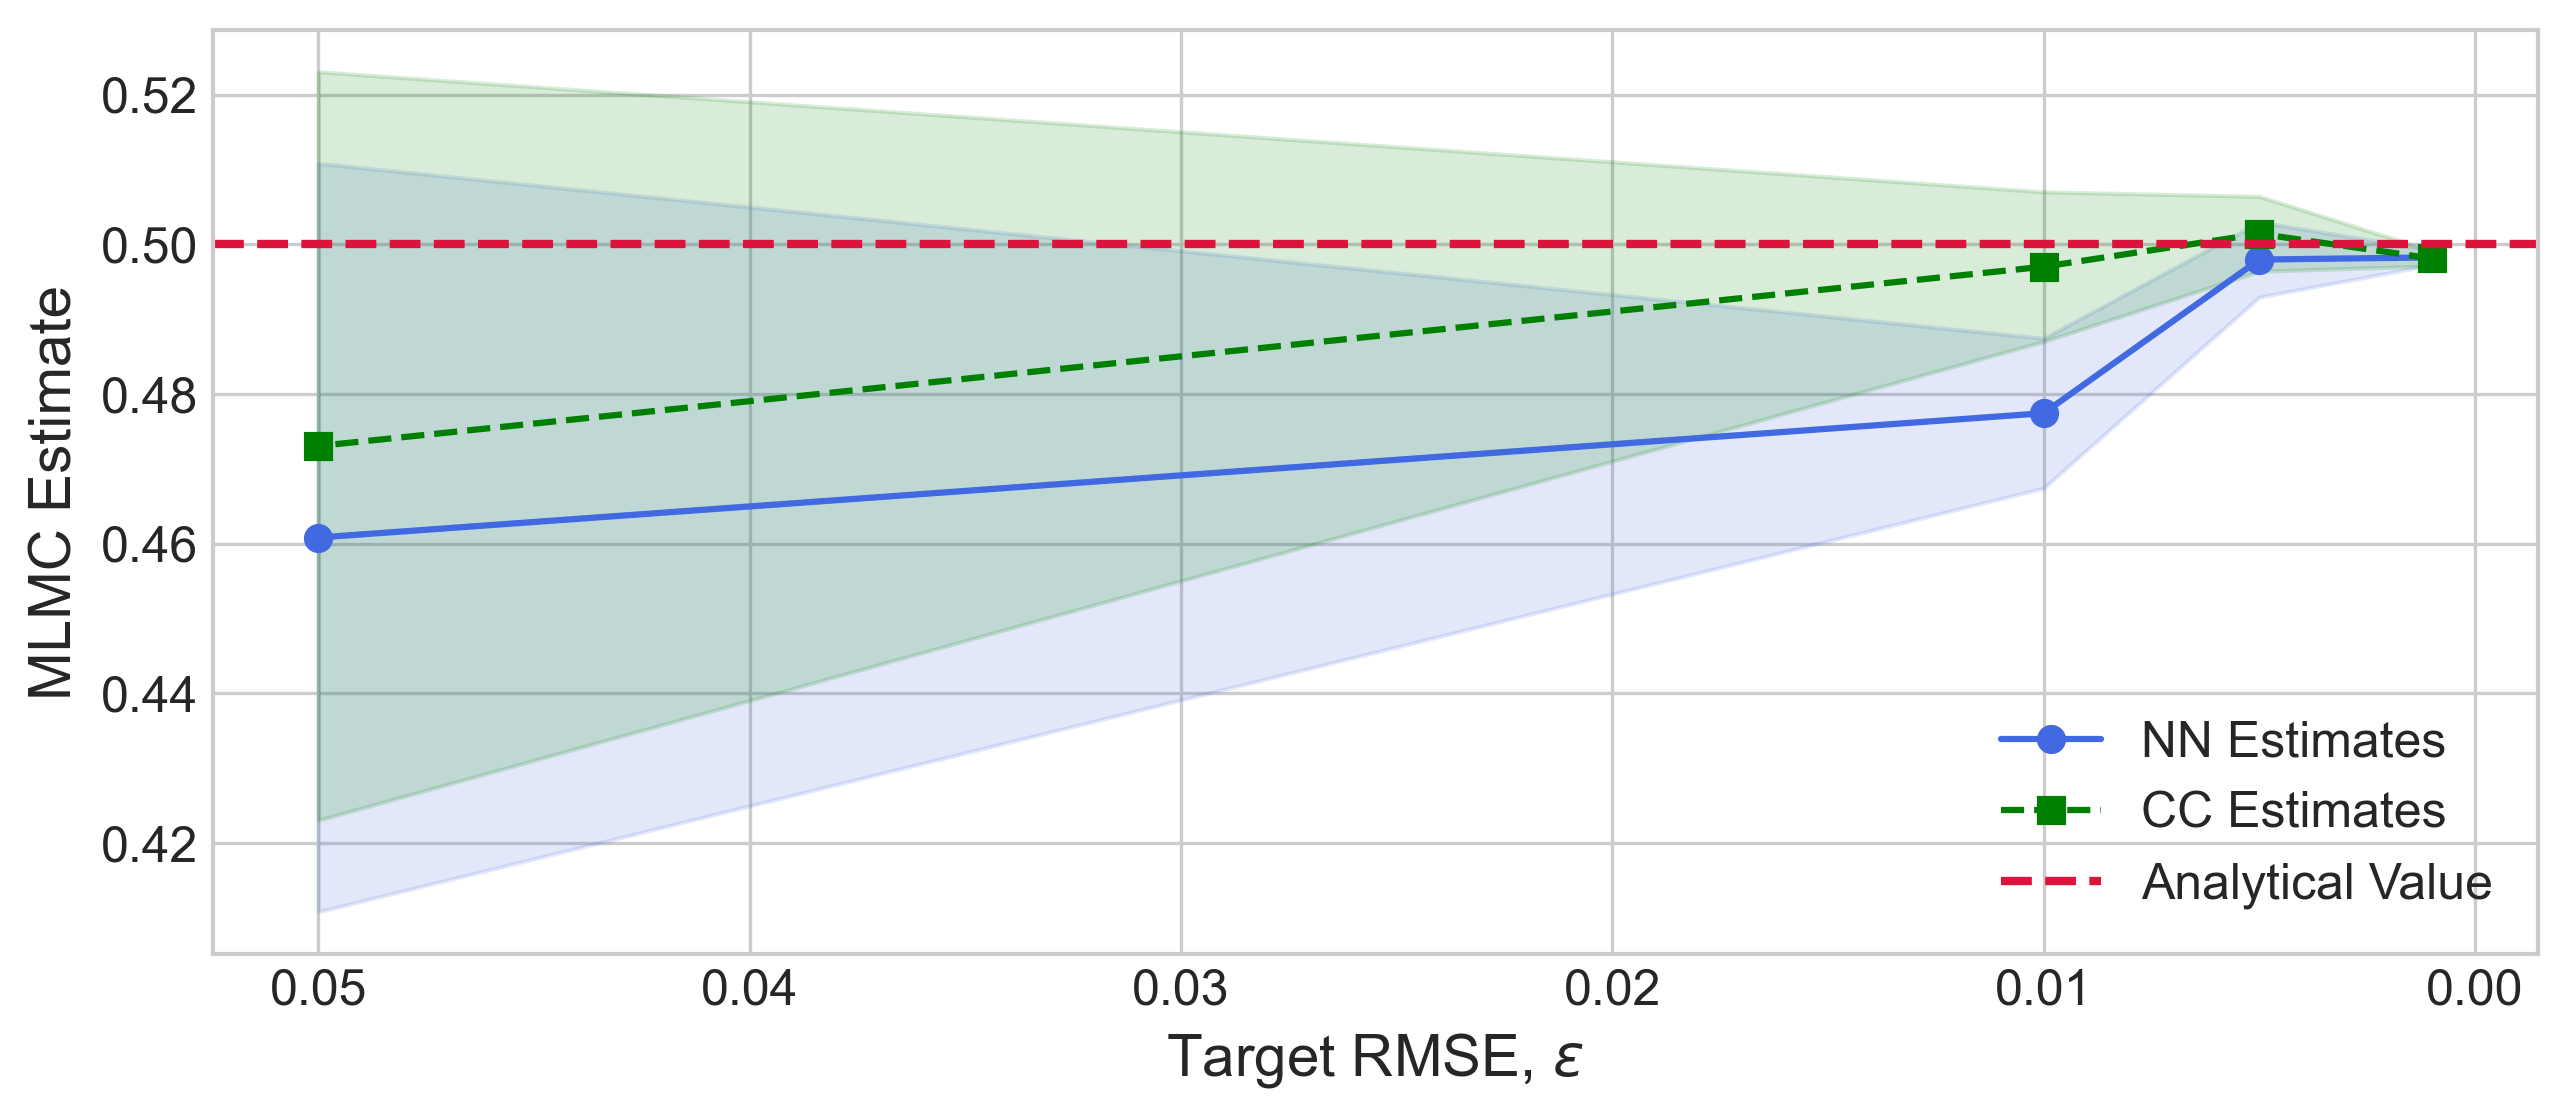
\includegraphics[width=0.7\linewidth]{graphics/dk_conv.png}
            \caption{Final MLMC estimate vs. target RMSE ($\varepsilon$).}
            \label{fig:conv_vs_eps}
        \end{subfigure}
        \vspace{0.5cm}
        \begin{subfigure}[b]{\textwidth}
            \centering
            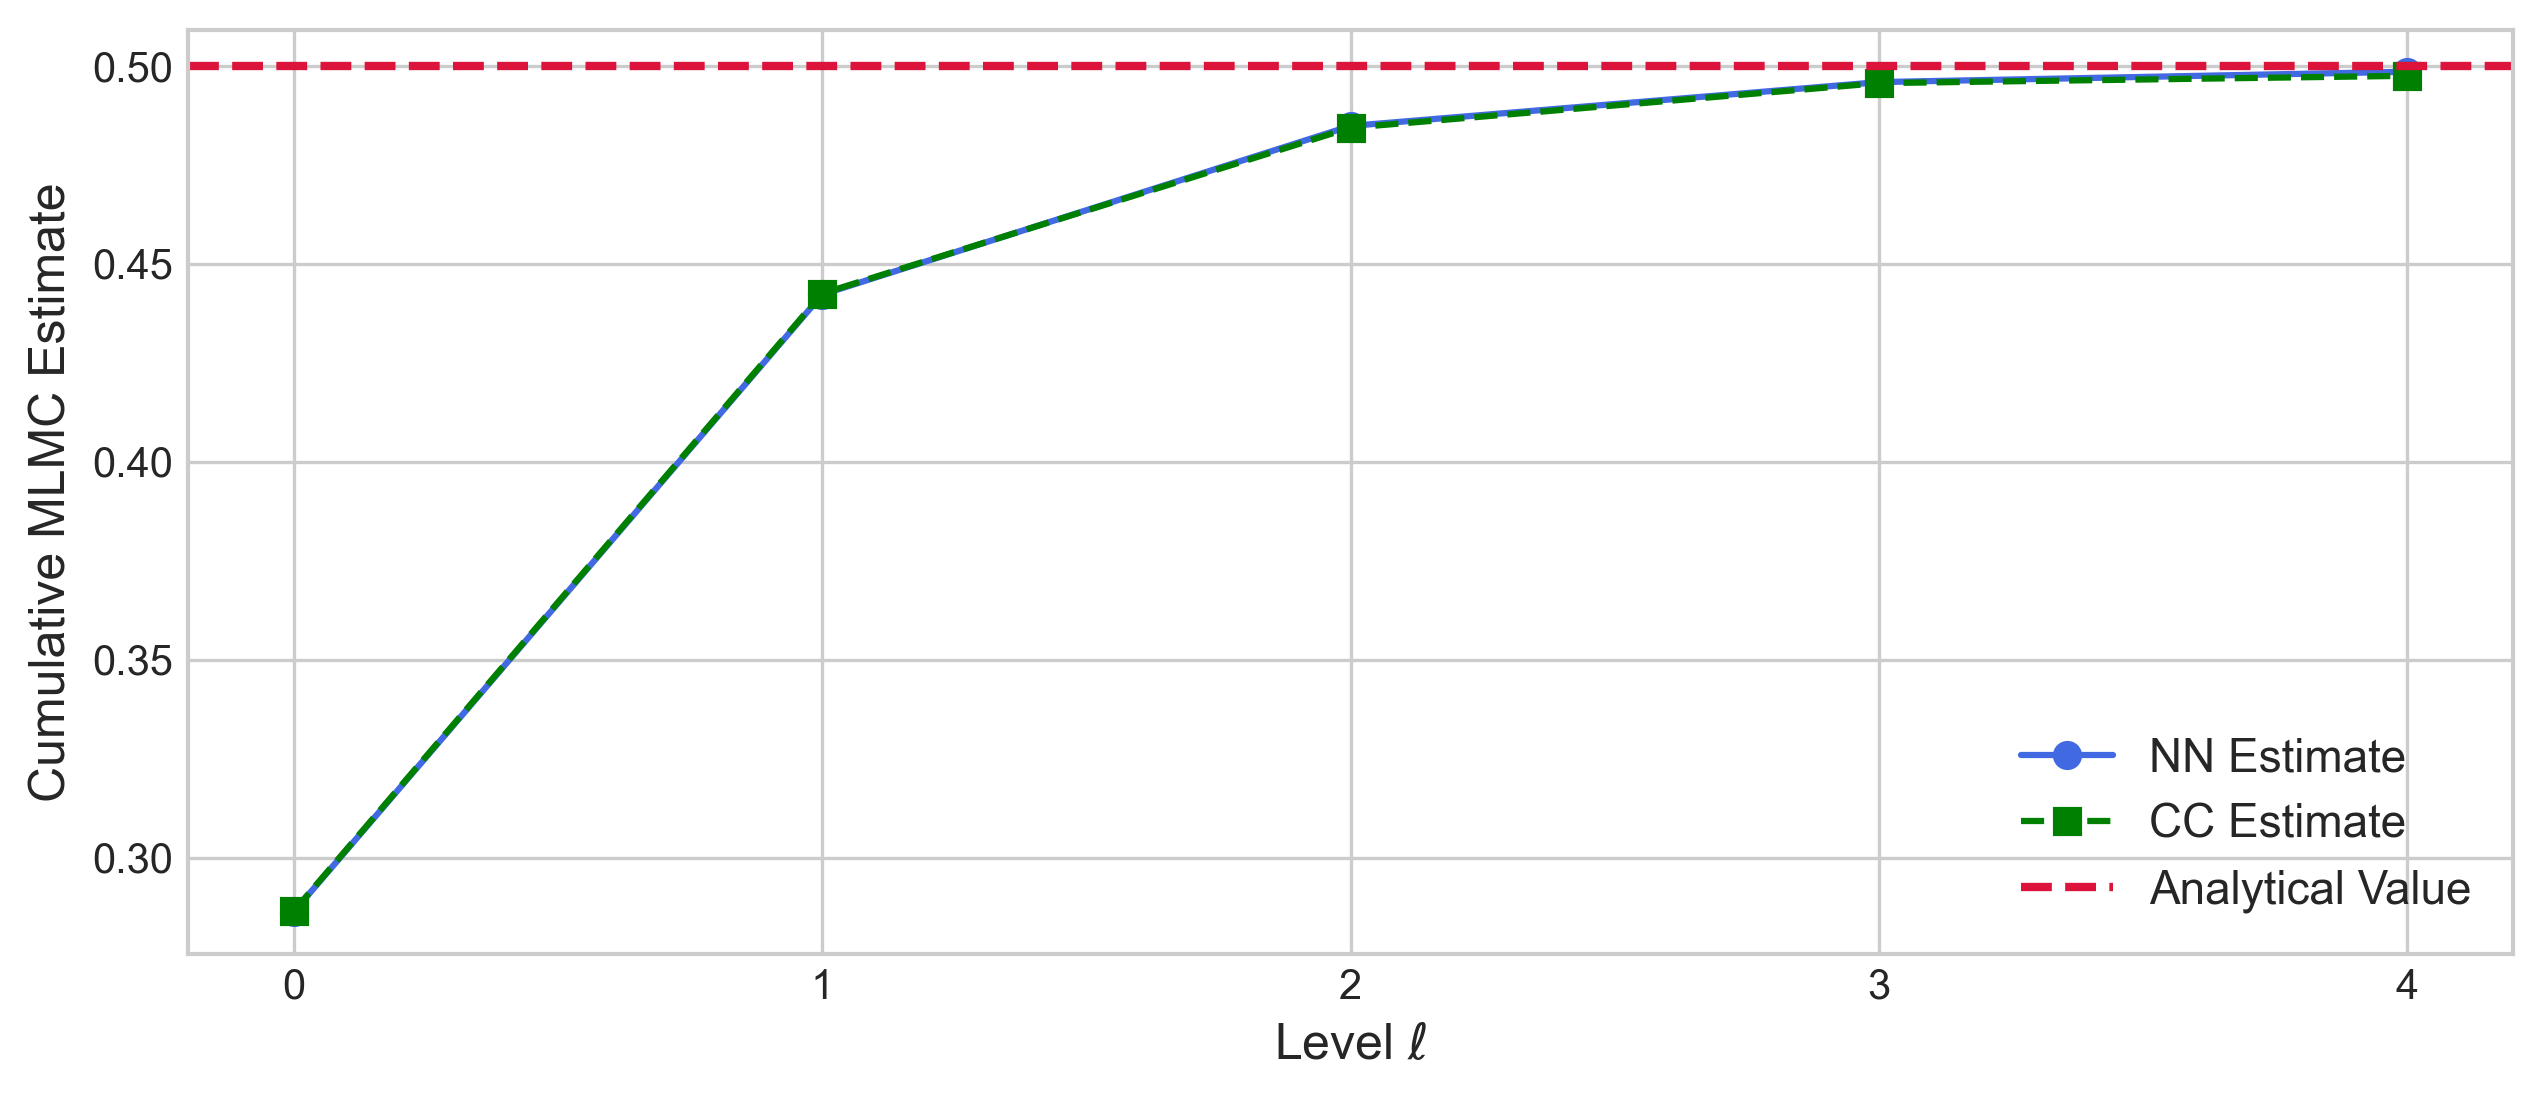
\includegraphics[width=0.7\linewidth]{graphics/dk_cumconv.png}
            \caption{Cumulative estimate vs. level ($\ell$) for $\varepsilon=0.001$.}
            \label{fig:cumulative_conv}
        \end{subfigure}
    \end{subfigure}
    \caption{Validation and convergence plots for the MLMC implementation for the Dean-Kawasaki equation.}
    \label{fig:she_validation_combined}
\end{figure}




% \include{conclusions}

%now enable appendix numbering format and include any appendices
\appendix
\include{appendix1}
\include{appendix2}

%next line adds the Bibliography to the contents page
\addcontentsline{toc}{chapter}{Bibliography}
%uncomment next line to change bibliography name to references
%\renewcommand{\bibname}{References}
\bibliography{refs}        %use a bibtex bibliography file refs.bib
\bibliographystyle{plain}  %use the plain bibliography style

\end{document}
